%Anomalies discovered and LaTeX hints are described at the bottom of this file.
\documentclass[letterpaper,10pt,titlepage]{custbook}
%
\pagestyle{headings}
%
\usepackage{amsmath}
\usepackage{amsfonts}
\usepackage{amssymb}
\usepackage[ansinew]{inputenc}
\usepackage[OT1]{fontenc}
\usepackage{graphicx}
\usepackage{longtable}
\usepackage{makeidx}
%
%Define certain conspicuous global constants.
\newcommand{\productbasenamelong}{Microcontroller Mathematical, Crytographic, and Utility Library}
\newcommand{\productbasenameshort}{UCULIB}
\newcommand{\productbasenameultrashort}{UCU}
\newcommand{\productversion}{0.0a}
\newcommand{\productname}{\productbasenameshort{}-\productversion}
%
%Used to correct bad typesetting of space after underscore.  No idea why
%this occurs.
\newcommand{\underscorepostspace}{\kern 0.1em}

%Used for non-breaking space between "Chapter" and the chapter number.
%With a stretchable space, it doesn't look quite right when the chapters
%are described individually and there are bullet points in a row but the
%chapter numbers don't line up.
\newcommand{\postchapterwordnonstretchable}{\kern 0.3333em}

%Embarrassingly, I've forgotten why "makeindex" is necessary ...
\makeindex
%
%Shared mathematical definitions
%%Sets of real numbers.
\newcommand{\vworkrealset}{{\mathbb{R}}}
\newcommand{\vworkrealsetnonneg}{{\mathbb{R}^+}}
%
%%Sets of integers.
\newcommand{\vworkintset}{{\mathbb{Z}}}
\newcommand{\vworkintsetnonneg}{{\mathbb{Z}^+}}
\newcommand{\vworkintsetpos}{{\mathbb{N}}}
%
%%Sets of rational numbers.
\newcommand{\vworkratset}{{\mathbb{Q}}}
\newcommand{\vworkratsetnonneg}{{\mathbb{Q}^+}}
%
%%Sets of irrational numbers.
\newcommand{\vworkirratset}{{\mathbb{error}}}
\newcommand{\vworkirratsetnonneg}{{\mathbb{error}^+}}
%
%%"Divides" and "Not Divides".  Am not able to find quite
%%the right symbol for "Not Divides" at this time.
\newcommand{\vworkdivides}{\mid}
\newcommand{\vworknotdivides}{\hspace{-0.125em}\not\hspace{0.245em}\mid\hspace{0.135em}}
%%
%%The implication operator, which may change throughout the work.  Both a horizontal
%%and vertical form are defined.
\newcommand{\vworkhimp}{\to}
\newcommand{\vworkvimp}{\downarrow}
%%
%%The symbol for logical equivalence.  There are three forms defined, the standard,
%%the long, and the short, which may be identical.
\newcommand{\vworkequiv}{\leftrightarrow}
\newcommand{\vworkshortequiv}{\leftrightarrow}
\newcommand{\vworklongequiv}{\longleftrightarrow}
\newcommand{\vworkvertequiv}{\updownarrow}

%
%Hyphenation exceptions
%This file contains hyphenation exceptions for work.
\hyphenation{EEPROM}
\hyphenation{MATLAB}
\hyphenation{SIMULINK}
\hyphenation{UPPAAL}

%
%New environments, etc.
%%%%%%%%%%%%%%%%%%%%%%%%%%%%%%%%%%%%%%%%%%%%%%%%%%%%%%%%%%%%%%%%%%%%%%%%%%%%%
%% SEPARATORS
%%%%%%%%%%%%%%%%%%%%%%%%%%%%%%%%%%%%%%%%%%%%%%%%%%%%%%%%%%%%%%%%%%%%%%%%%%%%%
%%
%Digit separation distance for denoting thousands, etc.  Choosing space rather than comma.
\newcommand{\vworkthousandsdigsepinmathmode}{\;}
%%
%%%%%%%%%%%%%%%%%%%%%%%%%%%%%%%%%%%%%%%%%%%%%%%%%%%%%%%%%%%%%%%%%%%%%%%%%%%%%
%% CHAPTER QUOTES
%%%%%%%%%%%%%%%%%%%%%%%%%%%%%%%%%%%%%%%%%%%%%%%%%%%%%%%%%%%%%%%%%%%%%%%%%%%%%
%%
%Quote which begins each chapter.
\newcommand{\beginchapterquote}[2]{\textbf{#1}\begin{flushright}\emph{---#2}\end{flushright}}

%Source when included with quote which begins each chapter.
\newcommand{\chapquoteshortsrc}[1]{\begin{flushright}\emph{---#1}\end{flushright}}
%%
%%%%%%%%%%%%%%%%%%%%%%%%%%%%%%%%%%%%%%%%%%%%%%%%%%%%%%%%%%%%%%%%%%%%%%%%%%%%%
%% EXAMPLES
%%%%%%%%%%%%%%%%%%%%%%%%%%%%%%%%%%%%%%%%%%%%%%%%%%%%%%%%%%%%%%%%%%%%%%%%%%%%%
%%
%General-purpose example start.  Used to generate the beginning of the example
%only, should enclose only an optional label.
\newtheorem{vworkgenexample}{Example}

%General-purpose example solution start.
\newcommand{\vworkgenexamplesolutionhead}{\noindent\textbf{Solution: }}

%General-purpose example solution body.  This is the environment in which
%the example's solution is stated.  For the present time, there are no
%changes to the text.
\newenvironment{vworkgenexamplesolutionbody}{\noindent\textbf{Solution: }}{}

%Define a new counter used to hold the example number within a chapter.
%\newcounter{vworkexamplecounter}[chapter]

%Alternate numbering for examples.
%\renewcommand{\thevworkexamplecounter}{\thechapter.\arabic{vworkexamplecounter}}

%Define the marking which delimits the start of an example.  For now, this
%is a little bit of space and a horizontal bar.
\newcommand{\vworkexampleheader}{\par\nopagebreak\vspace{0.01in}%
                                 \noindent\rule{\textwidth}{1pt}%
                                 \par\nopagebreak}

%Define the marking which delimits the end of an example.  For now, this is
%a horizontal line.  An example must be "footed" manually because there are
%so many variations on what can be in an example.
\newcommand{\vworkexamplefooter}{\par\nopagebreak%
                                 \vspace{0.01in}\noindent\rule{\textwidth}{1pt}%
                                 \par\nopagebreak}

%Define a new environment to hold the body of an example, and the numbering of an
%example.
\newenvironment{vworkexamplestatement}%
               {\vworkexampleheader\noindent%
               \setlength{\parindent}{0em}%
               \setlength{\parskip}{1ex}%
               \refstepcounter{vworktheoremcounter}%
               \textbf{Example \nopagebreak[2]\thevworktheoremcounter{}: }}{\par}

%Define a new environment to hold a "solution" or "remarks" block within an example.
%The presence or absence of a colon is something that may change, so better to code
%that in here.
\newenvironment{vworkexampleparsection}[1]{\par\noindent%
               \setlength{\parindent}{0em}%
               \setlength{\parskip}{1ex}%
               \textbf{#1:\nopagebreak[2] }}{\par}
%%
%%%%%%%%%%%%%%%%%%%%%%%%%%%%%%%%%%%%%%%%%%%%%%%%%%%%%%%%%%%%%%%%%%%%%%%%%%%%%
%% DEFINITIONS
%%%%%%%%%%%%%%%%%%%%%%%%%%%%%%%%%%%%%%%%%%%%%%%%%%%%%%%%%%%%%%%%%%%%%%%%%%%%%
%%
%Counter for "artifical" theorems.  In this context, "artificial" means that the
%built-in theorem environment is not used.
%\newcounter{vworkdefinitioncounter}[chapter]

%Alternate numbering for definitions.
%\renewcommand{\thevworkdefinitioncounter}{\thechapter.\arabic{vworkdefinitioncounter}}

%Define the markings which delimit the start and ends of a definition.  For now, these
%are NULL.  Later, I may define something else--a little extra space or a line.
\newcommand{\vworkdefinitionheader}{\par\nopagebreak%
                                    \vspace{0.01in}\noindent\rule{\textwidth}{1pt}%
                                    \par\nopagebreak}
\newcommand{\vworkdefinitionfooter}{\par\nopagebreak%
                                    \vspace{0.01in}\noindent\rule{\textwidth}{1pt}%
                                    \par\nopagebreak}

%Environment to hold definitions.  This was defined (rather than using the built-in
%environment) because I cannot stand having a number without a colon.
\newenvironment{vworkdefinitionstatement}%
               {\vworkdefinitionheader\noindent%
               \setlength{\parindent}{0em}%
               \setlength{\parskip}{1ex}%
               \refstepcounter{vworktheoremcounter}%
               \textbf{Definition \nopagebreak[2]\thevworktheoremcounter{}: }}{\par}

%Environment to begin a definition that also has descriptive text.
\newenvironment{vworkdefinitionstatementpar}[1]%
               {\vworkdefinitionheader\noindent%
               \setlength{\parindent}{0em}%
               \setlength{\parskip}{1ex}%
               \refstepcounter{vworktheoremcounter}%
               \textbf{Definition \nopagebreak[2]\thevworktheoremcounter{} (#1): }}{\par}

%Define a new environment to hold a "solution" or "remarks" block within a definition.
%The presence or absence of a colon is something that may change, so better to code
%that in here.
\newenvironment{vworkdefinitionparsection}[1]{\par\noindent%
               \setlength{\parindent}{0em}%
               \setlength{\parskip}{1ex}%
               \textbf{#1:\nopagebreak[2] }}{\par}
%%
%%%%%%%%%%%%%%%%%%%%%%%%%%%%%%%%%%%%%%%%%%%%%%%%%%%%%%%%%%%%%%%%%%%%%%%%%%%%%
%% LEMMAS
%%%%%%%%%%%%%%%%%%%%%%%%%%%%%%%%%%%%%%%%%%%%%%%%%%%%%%%%%%%%%%%%%%%%%%%%%%%%%
%%
%% Because lemmas and theorems are so similar, decided that they should
%% use the same counters.  I think this makes it easier for readers, so they
%% don't have to separate the two out when searching.
%%
%\newcounter{vworktheoremcounter}[chapter]

%Alternate numbering for lemmas.
%\renewcommand{\thevworktheoremcounter}{\thechapter.\arabic{vworktheoremcounter}}

%Define the markings which delimit the start and ends of a lemma.  For now, these
%are NULL.  Later, I may define something else--a little extra space or a line.
\newcommand{\vworklemmaheader}{\par\nopagebreak%
                               \vspace{0.01in}\noindent\rule{\textwidth}{1pt}%
                               \par\nopagebreak}
\newcommand{\vworklemmafooter}{\par\nopagebreak%
                               \vspace{0.01in}\noindent\rule{\textwidth}{1pt}%
                               \par\nopagebreak}

%Environment to hold lemmas.  This was defined (rather than using the built-in
%environment) because I cannot stand having a number without a colon.
\newenvironment{vworklemmastatement}%
               {\vworklemmaheader\noindent%
               \setlength{\parindent}{0em}%
               \setlength{\parskip}{1ex}%
               \refstepcounter{vworktheoremcounter}%
               \textbf{Lemma \nopagebreak[2]\thevworktheoremcounter{}: }}{\par}

%Environment to begin a lemma that also has descriptive text.
\newenvironment{vworklemmastatementpar}[1]%
               {\vworklemmaheader\noindent%
               \setlength{\parindent}{0em}%
               \setlength{\parskip}{1ex}%
               \refstepcounter{vworktheoremcounter}%
               \textbf{Lemma \nopagebreak[2]\thevworktheoremcounter{} (#1): }}{\par}

%Define a new environment to hold the proof of a lemma.
\newenvironment{vworklemmaproof}%
               {\par\noindent%
               \setlength{\parindent}{0em}%
               \setlength{\parskip}{1ex}%
               \textbf{Proof:\nopagebreak[2] }}{\hfill\rule{1.5ex}{1.5ex}\par}

%Define a new environment to hold a "solution" or "remarks" block within a lemma.
%The presence or absence of a colon is something that may change, so better to code
%that in here.
\newenvironment{vworklemmaparsection}[1]{\par\noindent%
               \setlength{\parindent}{0em}%
               \setlength{\parskip}{1ex}%
               \textbf{#1:\nopagebreak[2] }}{\par}
%%
%%%%%%%%%%%%%%%%%%%%%%%%%%%%%%%%%%%%%%%%%%%%%%%%%%%%%%%%%%%%%%%%%%%%%%%%%%%%%
%% THEOREMS
%%%%%%%%%%%%%%%%%%%%%%%%%%%%%%%%%%%%%%%%%%%%%%%%%%%%%%%%%%%%%%%%%%%%%%%%%%%%%
%%
%Counter for "artifical" theorems.  In this context, "artificial" means that the
%built-in theorem environment is not used.
\newcounter{vworktheoremcounter}[chapter]

%Alternate numbering for theorems.
\renewcommand{\thevworktheoremcounter}{\thechapter.\arabic{vworktheoremcounter}}

%Define the markings which delimit the start and ends of a theorem.  For now, these
%are NULL.  Later, I may define something else--a little extra space or a line.
\newcommand{\vworktheoremheader}{\par\nopagebreak%
                                 \vspace{0.01in}\noindent\rule{\textwidth}{1pt}%
                                 \par\nopagebreak}
\newcommand{\vworktheoremfooter}{\par\nopagebreak%
                                 \vspace{0.01in}\noindent\rule{\textwidth}{1pt}%
                                 \par\nopagebreak}

%Environment to hold theorems.  This was defined (rather than using the built-in
%environment) because I cannot stand having a number without a colon.
\newenvironment{vworktheoremstatement}%
               {\vworktheoremheader\noindent%
               \setlength{\parindent}{0em}%
               \setlength{\parskip}{1ex}%
               \refstepcounter{vworktheoremcounter}%
               \textbf{Theorem \nopagebreak[2]\thevworktheoremcounter{}: }}{\par}

%Environment to begin a theorem that also has descriptive text.
\newenvironment{vworktheoremstatementpar}[1]%
               {\vworktheoremheader\noindent%
               \setlength{\parindent}{0em}%
               \setlength{\parskip}{1ex}%
               \refstepcounter{vworktheoremcounter}%
               \textbf{Theorem \nopagebreak[2]\thevworktheoremcounter{} (#1): }}{\par}

%Define a new environment to hold the proof of a theorem.
\newenvironment{vworktheoremproof}%
               {\par\noindent%
               \setlength{\parindent}{0em}%
               \setlength{\parskip}{1ex}%
               \textbf{Proof:\nopagebreak[2] }}{\hfill\rule{1.5ex}{1.5ex}\par}

%Define a new environment to hold a "solution" or "remarks" block within a theorem.
%The presence or absence of a colon is something that may change, so better to code
%that in here.
\newenvironment{vworktheoremparsection}[1]{\par\noindent%
               \setlength{\parindent}{0em}%
               \setlength{\parskip}{1ex}%
               \textbf{#1:\nopagebreak[2] }}{\par}
%%
%%%%%%%%%%%%%%%%%%%%%%%%%%%%%%%%%%%%%%%%%%%%%%%%%%%%%%%%%%%%%%%%%%%%%%%%%%%%%
%% ALGORITHMS
%%%%%%%%%%%%%%%%%%%%%%%%%%%%%%%%%%%%%%%%%%%%%%%%%%%%%%%%%%%%%%%%%%%%%%%%%%%%%
%%
%Counter for "artifical" theorems.  In this context, "artificial" means that the
%built-in theorem environment is not used.
%\newcounter{vworktheoremcounter}[chapter]

%Alternate numbering for theorems.
%\renewcommand{\thevworktheoremcounter}{\thechapter.\arabic{vworktheoremcounter}}

%Define the markings which delimit the start and ends of an algorithm.  For now, these
%are NULL.  Later, I may define something else--a little extra space or a line.
\newcommand{\vworkalgorithmheader}{\par\nopagebreak%
                                 \vspace{0.01in}\noindent\rule{\textwidth}{1pt}%
                                 \par\nopagebreak}
\newcommand{\vworkalgorithmfooter}{\par\nopagebreak%
                                 \vspace{0.01in}\noindent\rule{\textwidth}{1pt}%
                                 \par\nopagebreak}

%Environment to hold algorithms.  This was defined (rather than using the built-in
%environment) because I cannot stand having a number without a colon.
\newenvironment{vworkalgorithmstatement}%
               {\vworkalgorithmheader\noindent%
               \setlength{\parindent}{0em}%
               \setlength{\parskip}{1ex}%
               \refstepcounter{vworktheoremcounter}%
               \textbf{Algorithm \nopagebreak[2]\thevworktheoremcounter{}: }}{\par}

%Environment to begin an algorithm that also has descriptive text.
\newenvironment{vworkalgorithmstatementpar}[1]%
               {\vworkalgorithmheader\noindent%
               \setlength{\parindent}{0em}%
               \setlength{\parskip}{1ex}%
               \refstepcounter{vworktheoremcounter}%
               \textbf{Algorithm \nopagebreak[2]\thevworktheoremcounter{} (#1): }}{\par}

%Define a new environment to hold the proof of an algorithm.
\newenvironment{vworkalgorithmproof}%
               {\par\noindent%
               \setlength{\parindent}{0em}%
               \setlength{\parskip}{1ex}%
               \textbf{Proof:\nopagebreak[2] }}{\hfill\rule{1.5ex}{1.5ex}\par}

%Define a new environment to hold a "solution" or "remarks" block within an algorithm.
%The presence or absence of a colon is something that may change, so better to code
%that in here.
\newenvironment{vworkalgorithmparsection}[1]{\par\noindent%
               \setlength{\parindent}{0em}%
               \setlength{\parskip}{1ex}%
               \textbf{#1:\nopagebreak[2] }}{\par}
%The "itemize" environment defined by the book style files didn't seem to have
%quite the right appearance for presenting our algorithms.  For this reason, the
%following environments were defined.  Level 0 is flush left with bullets, Level 1
%is slightly more indented, etc.
\newenvironment{alglvl0}{\begin{list}
               {$\bullet$}{\setlength{\labelwidth}{3mm}\setlength{\leftmargin}{6mm}}}
               {\end{list}}
\newenvironment{alglvl1}{\begin{list}
               {$\bullet$}{\setlength{\labelwidth}{3mm}\setlength{\leftmargin}{6mm}}}
               {\end{list}}
\newenvironment{alglvl2}{\begin{list}
               {$\bullet$}{\setlength{\labelwidth}{3mm}\setlength{\leftmargin}{6mm}}}
               {\end{list}}
%The environments above have been obsoleted.
\newcounter{alglvl0ctr}
\newenvironment{algblvl0}{\begin{list}
               {\textbf{[\arabic{alglvl0ctr}]}}{\usecounter{alglvl0ctr}%
               \setlength{\labelwidth}{6mm}\setlength{\leftmargin}{9mm}}}
               {\end{list}}
%%
%%%%%%%%%%%%%%%%%%%%%%%%%%%%%%%%%%%%%%%%%%%%%%%%%%%%%%%%%%%%%%%%%%%%%%%%%%%%%
%% EXERCISES
%%%%%%%%%%%%%%%%%%%%%%%%%%%%%%%%%%%%%%%%%%%%%%%%%%%%%%%%%%%%%%%%%%%%%%%%%%%%%
%%
%Counter for exercises at the end of each chapter.
\newcounter{vworkexercisecounter}[chapter]

%We'd like to number an exercise slightly differently, using the chapter number
%followed by "." followed by the equation number.
\renewcommand{\thevworkexercisecounter}{\thechapter.\arabic{vworkexercisecounter}}

%Define the markings which delimit the start and ends of an exercise.  For now, these
%are NULL.  Later, I may define something else--a little extra space or a line.
\newcommand{\vworkexerciseheader}{\par\vspace{0.01in}\par}
\newcommand{\vworkexercisefooter}{\par\vspace{0.01in}\par}

%Environment to hold exercises.
\newenvironment{vworkexercisestatement}%
               {\vworkexerciseheader\noindent%
               \setlength{\parindent}{0em}%
               \setlength{\parskip}{1ex}%
               \refstepcounter{vworkexercisecounter}%
               \textbf{[\thevworkexercisecounter{}]}\nopagebreak[2] }{\par}

%Define a new environment to hold a "remarks" block within an exercise.
%The presence or absence of a colon is something that may change, so better to code
%that in here.
\newenvironment{vworkexerciseparsection}[1]{\par\noindent%
               \setlength{\parindent}{0em}%
               \setlength{\parskip}{1ex}%
               \textbf{#1: }}{\par}
%%
%%%%%%%%%%%%%%%%%%%%%%%%%%%%%%%%%%%%%%%%%%%%%%%%%%%%%%%%%%%%%%%%%%%%%%%%%%%%%
%% LESSONS LEARNED
%%%%%%%%%%%%%%%%%%%%%%%%%%%%%%%%%%%%%%%%%%%%%%%%%%%%%%%%%%%%%%%%%%%%%%%%%%%%%
%%
%Counter for lessons learned.
\newcounter{vworklessonslearnedcounter}[chapter]

%Alternate numbering for lessons learned.
\renewcommand{\thevworklessonslearnedcounter}{\thechapter.\arabic{vworklessonslearnedcounter}}

%Define the markings which delimit the start and ends of a lesson learned.
\newcommand{\vworklessonslearnedheader}{\par\nopagebreak%
                                 \vspace{0.01in}\noindent\rule{\textwidth}{1pt}%
                                 \par\nopagebreak}
\newcommand{\vworklessonslearnedfooter}{\par\nopagebreak%
                                 \vspace{0.01in}\noindent\rule{\textwidth}{1pt}%
                                 \par\nopagebreak}

%Environment to hold lessons learned.
\newenvironment{vworklessonslearnedstatement}%
               {\vworklessonslearnedheader\noindent%
               \setlength{\parindent}{0em}%
               \setlength{\parskip}{1ex}%
               \refstepcounter{vworklessonslearnedcounter}%
               \textbf{Lesson Learned \nopagebreak[2]\thevworklessonslearnedcounter{}: }}{\par}
%%
%%%%%%%%%%%%%%%%%%%%%%%%%%%%%%%%%%%%%%%%%%%%%%%%%%%%%%%%%%%%%%%%%%%%%%%%%%%%%
%% QUOTES
%%%%%%%%%%%%%%%%%%%%%%%%%%%%%%%%%%%%%%%%%%%%%%%%%%%%%%%%%%%%%%%%%%%%%%%%%%%%%
%%
%Environment to hold quotes.
\newenvironment{indentedquote}{\begin{quote}}{\end{quote}}
%%
%%%%%%%%%%%%%%%%%%%%%%%%%%%%%%%%%%%%%%%%%%%%%%%%%%%%%%%%%%%%%%%%%%%%%%%%%%%%%
%% EXERCISE SOLUTIONS
%%%%%%%%%%%%%%%%%%%%%%%%%%%%%%%%%%%%%%%%%%%%%%%%%%%%%%%%%%%%%%%%%%%%%%%%%%%%%
%%
%Environment To Hold A Solution To An Exercise
\newenvironment{vworkexercisesolution}[1]{\par\noindent%
               \setlength{\parindent}{0em}%
               \setlength{\parskip}{1ex}%
               \textbf{Solution To Exercise #1}\par}{\par}

%Command which begins section of solutions for each chapter, command which
%separates solutions, and command which ends solutions in each chapter.
\newcommand{\vworkexercisechapterheader}{\par\nopagebreak\vspace{0.01in}%
                                 \noindent\rule{\textwidth}{1pt}%
                                 \par\nopagebreak}
\newcommand{\vworkexerciseseparator}{\par\nopagebreak\vspace{0.01in}%
                                 \noindent\rule{\textwidth}{1pt}%
                                 \par\nopagebreak}
\newcommand{\vworkexercisechapterfooter}{\par\nopagebreak%
                                 \vspace{0.01in}\noindent\rule{\textwidth}{1pt}%
                                 \par\nopagebreak}
%%
%%%%%%%%%%%%%%%%%%%%%%%%%%%%%%%%%%%%%%%%%%%%%%%%%%%%%%%%%%%%%%%%%%%%%%%%%%%%%
%% GLOSSARY OF TERMS
%%%%%%%%%%%%%%%%%%%%%%%%%%%%%%%%%%%%%%%%%%%%%%%%%%%%%%%%%%%%%%%%%%%%%%%%%%%%%
%5
%The following environment is for the glossary of terms at the end.
\newenvironment{vworktermglossaryenum}{\begin{list}
               {}{\setlength{\labelwidth}{0mm}
                  \setlength{\leftmargin}{4mm}
                  \setlength{\itemindent}{-4mm}
                  \setlength{\parsep}{0.85mm}}}
               {\end{list}}
%%
%%%%%%%%%%%%%%%%%%%%%%%%%%%%%%%%%%%%%%%%%%%%%%%%%%%%%%%%%%%%%%%%%%%%%%%%%%%%%
%% GLOSSARY OF MATHEMATICAL TERMS
%%%%%%%%%%%%%%%%%%%%%%%%%%%%%%%%%%%%%%%%%%%%%%%%%%%%%%%%%%%%%%%%%%%%%%%%%%%%%
%%
%The following environment is for the glossary of mathematical terms at the end.
\newenvironment{vworkmathtermglossaryenum}{\begin{list}
               {}{\setlength{\labelwidth}{0mm}
                  \setlength{\leftmargin}{4mm}
                  \setlength{\itemindent}{-4mm}
                  \setlength{\parsep}{0.85mm}}}
               {\end{list}}

%%%%%%%%%%%%%%%%%%%%%%%%%%%%%%%%%%%%%%%%%%%%%%%%%%%%%%%%%%%%%%%%%%%%%%%%%%%%%%%%%%%%%%%%%%
%%%%%%%%%%%%%%%%%%%%%%%%%%%%%%%%%%%%%%%%%%%%%%%%%%%%%%%%%%%%%%%%%%%%%%%%%%%%%%%%%%%%%%%%%%
% TCL COMMAND DOCUMENTATION
%
%Environment to hold the "NAME" portion of a Tcl command description.
\newenvironment{tclcommandname}[1]{\noindent\textbf{NAME}\vspace{-1.0ex}\begin{list}%
               {}{\setlength{\leftmargin}{0.25in}}\item\textbf{#1}---}{\end{list}}

%Command to display a synopsis line inside the synopsis environment.
\newcommand{\tclcommandsynopsisline}[2]{\par\textbf{#1} \textit{#2}\par}

%Environment to hold the "SYNOPSIS" portion of a Tcl command description.
\newenvironment{tclcommandsynopsis}{\noindent\textbf{SYNOPSIS}\vspace{-1.0ex}\begin{list}%
               {}{\setlength{\leftmargin}{0.25in}}\item{}}{\end{list}}

%Environment to hold the "DESCRIPTION" portion of a Tcl command description.
\newenvironment{tclcommanddescription}{\noindent\textbf{DESCRIPTION}\vspace{-1.0ex}\begin{list}%
               {}{\setlength{\leftmargin}{0.25in}}\item{}}{\end{list}}

%Environment to hold the "ACKNOWLEDGEMENTS" portion of a Tcl command description.
\newenvironment{tclcommandacknowledgements}{\noindent\textbf{ACKNOWLEDGEMENTS}\vspace{-1.0ex}\begin{list}%
               {}{\setlength{\leftmargin}{0.25in}}\item{}}{\end{list}}

%Environment to hold a specific subdescription within the DESCRIPTION--useful for enumerating
%possible legal commands and command forms.
\newenvironment{tclcommandinternaldescription}{\noindent{}\vspace{-5.0ex}\begin{list}%
               {}{\setlength{\leftmargin}{0.25in}}\item{}}{\end{list}}

%Command to use to format a command prototype preceding the environment above (i.e. a synopsis).
\newcommand{\tclcommanddescsynopsisline}[2]{\par\textbf{#1} \textit{#2}\par}

%Environment to hold the "USAGE NOTES" portion of a Tcl command description.
\newenvironment{tclcommandusagenotes}{\noindent\textbf{USAGE NOTES}\vspace{-1.0ex}\begin{list}%
               {}{\setlength{\leftmargin}{0.25in}}\item{}}{\end{list}}

%Environment to hold the "SAMPLE INVOCATIONS" portion of a TCL command or extension description.
\newenvironment{tclcommandsampleinvocations}{\noindent\textbf{SAMPLE INVOCATIONS}\vspace{-1.0ex}\begin{list}%
               {}{\setlength{\leftmargin}{0.25in}}\item{}}{\end{list}}

%Environment to hold the "SEE ALSO" portion of a TCL command or extension utility description.
\newenvironment{tclcommandseealso}{\noindent\textbf{SEE ALSO}\vspace{-1.0ex}\begin{list}%
               {}{\setlength{\leftmargin}{0.25in}}\item{}}{\end{list}}

%%%%%%%%%%%%%%%%%%%%%%%%%%%%%%%%%%%%%%%%%%%%%%%%%%%%%%%%%%%%%%%%%%%%%%%%%%%%%%%%%%%%%%%%%%
%%%%%%%%%%%%%%%%%%%%%%%%%%%%%%%%%%%%%%%%%%%%%%%%%%%%%%%%%%%%%%%%%%%%%%%%%%%%%%%%%%%%%%%%%%
% DOS COMMAND-LINE UTILITY DOCUMENTATION
%
%Environment to hold the "NAME" portion of a DOS command-line utility.
\newenvironment{dosutilcommandname}[1]{\noindent\textbf{NAME}\vspace{-1.0ex}\begin{list}%
               {}{\setlength{\leftmargin}{0.25in}}\item\textbf{#1}---}{\end{list}}

%Command to display a synopsis line inside the synopsis environment.
\newcommand{\dosutilcommandsynopsisline}[2]{\par\textbf{#1} \textit{#2}\par}

%Environment to hold the "SYNOPSIS" portion of a DOS command-line utility description.
\newenvironment{dosutilcommandsynopsis}{\noindent\textbf{SYNOPSIS}\vspace{-1.0ex}\begin{list}%
               {}{\setlength{\leftmargin}{0.25in}}\item{}}{\end{list}}

%Environment to hold the "DESCRIPTION" portion of a DOS command-line utility description.
\newenvironment{dosutilcommanddescription}{\noindent\textbf{DESCRIPTION}\vspace{-1.0ex}\begin{list}%
               {}{\setlength{\leftmargin}{0.25in}}\item{}}{\end{list}}

%Environment to hold the "ACKNOWLEDGEMENTS" portion of a DOS command-line utility description.
\newenvironment{dosutilcommandacknowledgements}{\noindent\textbf{ACKNOWLEDGEMENTS}\vspace{-1.0ex}\begin{list}%
               {}{\setlength{\leftmargin}{0.25in}}\item{}}{\end{list}}

%Environment to hold a specific subdescription within the DESCRIPTION--useful for enumerating
%possible legal commands and command forms.
\newenvironment{dosutilcommandinternaldescription}{\noindent{}\vspace{-5.0ex}\begin{list}%
               {}{\setlength{\leftmargin}{0.25in}}\item{}}{\end{list}}

%Command to use to format a command prototype preceding the environment above (i.e. a synopsis).
\newcommand{\dosutilcommanddescsynopsisline}[2]{\par\textbf{#1} \textit{#2}\par}

%Environment to hold the "USAGE NOTES" portion of a DOS command-line utility description.
\newenvironment{dosutilcommandusagenotes}{\noindent\textbf{USAGE NOTES}\vspace{-1.0ex}\begin{list}%
               {}{\setlength{\leftmargin}{0.25in}}\item{}}{\end{list}}

%Environment to hold the "REMARKS" portion of a DOS command-line utility description.
\newenvironment{dosutilcommandremarks}{\noindent\textbf{REMARKS}\vspace{-1.0ex}\begin{list}%
               {}{\setlength{\leftmargin}{0.25in}}\item{}}{\end{list}}

%Environment to hold the "COMMAND-LINE OPTIONS" portion of a DOS command-line utility description.
\newenvironment{dosutilcommandcommandlineoptions}{\noindent\textbf{COMMAND-LINE OPTIONS}\vspace{-1.0ex}\begin{list}%
               {}{\setlength{\leftmargin}{0.25in}}\item{}}{\end{list}}

%Environment to hold the "SAMPLE INVOCATION" portion of a DOS command-line utility description.
\newenvironment{dosutilcommandsampleinvocations}{\noindent\textbf{SAMPLE INVOCATIONS}\vspace{-1.0ex}\begin{list}%
               {}{\setlength{\leftmargin}{0.25in}}\item{}}{\end{list}}

%Environment to hold the "SEE ALSO" portion of a DOS command-line utility description.
\newenvironment{dosutilcommandseealso}{\noindent\textbf{SEE ALSO}\vspace{-1.0ex}\begin{list}%
               {}{\setlength{\leftmargin}{0.25in}}\item{}}{\end{list}}
%%
%%%%%%%%%%%%%%%%%%%%%%%%%%%%%%%%%%%%%%%%%%%%%%%%%%%%%%%%%%%%%%%%%%%%%%%%%%%%%
%% DESIRABLE PROPERTIES
%%%%%%%%%%%%%%%%%%%%%%%%%%%%%%%%%%%%%%%%%%%%%%%%%%%%%%%%%%%%%%%%%%%%%%%%%%%%%
%Command to identify the prefix used for desirable properties.
%"DP" seems as good as anything.
\newcommand{\desirablepropertyprefix}{DP}
%
%% This counter is used only to number the desirable properties of
%% embedded software used in the "Holy Grail" chapter.
\newcounter{vworkdesirablepropertiescounter}

%Command to increment the desirable properties counter, emit the tag,
%and set the \ref value.
\newcommand{\desirablepropertyemit}{\refstepcounter{vworkdesirablepropertiescounter}%
                                    [\desirablepropertyprefix-\thevworkdesirablepropertiescounter]}

%Command to cite a desirable property.
\newcommand{\desirablepropertycite}[1]{[\desirablepropertyprefix-\ref{#1}]}

%%%%%%%%%%%%%%%%%%%%%%%%%%%%%%%%%%%%%%%%%%%%%%%%%%%%%%%%%%%%%%%%%%%%%%%%%%%%%%%%%%%%%%%%%%
%%%%%%%%%%%%%%%%%%%%%%%%%%%%%%%%%%%%%%%%%%%%%%%%%%%%%%%%%%%%%%%%%%%%%%%%%%%%%%%%%%%%%%%%%%
%%%%%%%%%%%%%%%%%%%%%%%%%%%%%%%%%%%%%%%%%%%%%%%%%%%%%%%%%%%%%%%%%%%%%%%%%%%%%%%%%%%%%%%%%%

%
\begin{document}
%
%"See" definitions for the index.
\index{---ceiling@$\lceil  \cdot \rceil$|see{ceiling function}}
\index{---floor@$\lfloor \cdot \rfloor$|see{floor function}}
\index{---divides@$\vworkdivides$|see{divides}}
\index{---divides@$\vworknotdivides$|see{divides}}
\index{2's complement|see{two's complement}}
\index{ABI|see{application binary interface}}
\index{ASMP|see{asymmetric multiprocessor}}
\index{cardinality|see{set cardinality}}
\index{Donald E. Knuth|see{Knuth, Donald E.}}
\index{fetch|see{instruction fetch}}
\index{Leslie Lamport|see{Lamport, Leslie}}
\index{OOE|see{out-of-order execution}}
\index{retirement|see{instruction retirement}}
\index{SMP|see{symmetric multiprocessor}}
%
%Title page(s)
\thispagestyle{empty}

\begin{flushright}
\vspace*{0mm}
\huge\bfseries
\emph{\productbasenamelong{} (\productbasenameshort{})}\\
\emph{Version \productversion{}}\\
\end{flushright}
\vspace{0.0cm}
\noindent\rule{\textwidth}{2pt}
\begin{flushright}
\LARGE\bfseries
Design, Development, and User Manual
\end{flushright}
\vfill
\begin{flushright}
\begin{small}
David T. Ashley
\end{small}
\end{flushright}
\vspace{0.2cm}
\begin{flushright}
\begin{small}
Compiled from \LaTeX{} source code on \today .  
\end{small}
\end{flushright}

\pagebreak
\thispagestyle{empty}
\begin{centering}
This page intentionally left blank.
\end{centering}
\vfill

%
%Declare this as frontmatter, the front portion before the meat
%of the book.
\frontmatter{}
%
%Table of contents
\tableofcontents
%
%List of tables
\listoftables
%
%List of figures
\listoffigures
%
%Everything after this is the main matter, the "meat"
%of the book.
\mainmatter{}
%
% Part: General Information
\part{General Information}

% Chapter: Introduction and Overview
\chapter{Introduction and Overview}
\label{ciov0}

%%%%%%%%%%%%%%%%%%%%%%%%%%%%%%%%%%%%%%%%%%%%%%%%%%%%%%%%%%%%%%%%%%%%%%%%%%%%%%%
%%%%%%%%%%%%%%%%%%%%%%%%%%%%%%%%%%%%%%%%%%%%%%%%%%%%%%%%%%%%%%%%%%%%%%%%%%%%%%%
%%%%%%%%%%%%%%%%%%%%%%%%%%%%%%%%%%%%%%%%%%%%%%%%%%%%%%%%%%%%%%%%%%%%%%%%%%%%%%%
\section{Overview of the Library}
\label{ciov0:sdpr0}

%LaTeX won't substitute into \index{} below, so had to use the expanded
%name.
\index{UCULIB@\emph{UCULIB}}The library described in this 
document, the \emph{\productbasenamelong{}, Version 
\productversion{}} (identified more compactly as 
\emph{\productbasenameshort{}-\productversion{}}, 
\emph{\productbasenameshort{}}, or 
\emph{\productbasenameultrashort{}}) is a 
\emph{C}/\emph{C++}-callable 
arithmetic/mathematical/cryptographic software library for 
microcontrollers and embedded systems.  

The library includes functionality for: 

\begin{itemize}
\item \emph{Arithmetic:} native/\-large integer/\-fixed-point/\-large fixed-point/\-floating-point
      addition/\-sub\-tract\-ion/\-mul\-ti\-pli\-cat\-ion/\-division.
\item \emph{Mathematical algorithms:}
      native/\-large integer/\-fixed-point/\-large fixed-point/\-floating-point
      vector arithmetic, algebraic/transcendental functions.
\item \emph{Control system elements and linear filtering:}
      low/high-pass filtering, scaling, differentiation, integration.
\item \emph{Non-linear filtering:}
      discrete input debouncing, vertical counters.
\item \emph{Non-cryptographic hashes:}
      checksums, CRC's.
\item \emph{Cryptographic hashes:}
      hashes from the SHA-2 family (SHA-224, SHA-256, SHA-384, SHA-512, SHA-512/224, SHA-512/256).
\item \emph{Cryptography:}
      ciphers, PRNGs.
\item \emph{Bit-mapped sets:}
      union, intersection, cardinality, iteration.
\item \emph{Utility:}
      block memory
      operations, array operations.
\end{itemize}

\emph{\productbasenameshort{}} is a traditional
library in that:

\begin{itemize}
\item The source code is arranged as one function or data structure per source file.
\item The source code is compiled as one function or data structure per object file.
\item Object files are combined together into a library.
\item The linker extracts only what it needs to resolve references.  (This generally
      gives minimum FLASH and RAM footprint.)
\end{itemize}

\emph{\productbasenameshort{}} is similar in spirit to 
existing libraries such as \emph{The GNU Multiple Precision 
Arithmetic Library}\footnote{Hereinafter called \emph{The 
GMP} or \emph{GMP}.}, but it has some differences that make 
it more suitable for embedded software.  The features and 
characteristics of the \emph{\productbasenameshort{}} are: 

\begin{itemize}
\item The library is optimized for speed (similar to \emph{The GMP}).
      (Assembly-language for common
      processor variants is provided, with a slower C fallback.  Fixed-size operands
      allow complete loop-unrolling in many cases.)
\item The library seeks to use FLASH memory as economically as possible.  (The design
      of the library allows the linker to extract the minimum required, and the code is
      compacted as much as possible without materially sacrificing speed.)
\item The library seeks to use RAM as economically as possible (but when a speed/RAM
      tradeoff exists, speed is chosen so long as the RAM cost is not unreasonable).
\item Dynamic memory allocation is not used within the library
      (unlike \emph{The GMP}).\footnote{It is still
      possible for the library to operate using dynamically-allocated memory,
      but this memory must be obtained and released by the caller.}
\item All functions in the library operate on operands of a size known by the
      caller, and this data size does not change as a result of any
      library function (unlike \emph{The GMP}).\footnote{All functions
      either accept operands of a fixed
      size characteristic of the function, or accept a measure of size
      as a formal parameter.}
\item The source code for each library variant is created from templates,
      so that the source code contains almost no C preprocessor
      switches.  (The source code is arranged in this way for
      easier debugging,\footnote{Some source-level debuggers are
      confused by complex preprocessor switches.} and to remove uncertainty about what has
      is actually being compiled or assembled.)
\item The library can be repackaged as three source files (a \emph{.h} header file, a \emph{.c}
      source file, and an assembly-language file with a target-specific file extension),
      and used as two software modules within a project rather than as a library.\footnote{The
      library source code is designed to be used in this way because some debugging tools
      are awkward at debugging libraries.}\textsuperscript{,}\footnote{These three files are created automatically
      by the generator program, but it would take typically take substantial manual editing to
      eliminate unused functions and data structures from these files so that the FLASH footprint
      is the same as if a library is used.}
\item The library is made available only as source code.\footnote{The user must
      have the software tools necessary to compile the source code and create a
      library.}
\item The library is thread-safe and core-safe.
\item The library is designed to be used on multi-core processors without
      a cache coherency protocol.\footnote{However, the library achieves this by
      requiring the caller to perform all necessary cache line invalidations
      and flushes.}
\item The library is unit tested to MC/DC coverage, and is 
      expected to contain no software defects.  
\end{itemize}


%%%%%%%%%%%%%%%%%%%%%%%%%%%%%%%%%%%%%%%%%%%%%%%%%%%%%%%%%%%%%%%%%%%%%%%%%%%%%%%
%%%%%%%%%%%%%%%%%%%%%%%%%%%%%%%%%%%%%%%%%%%%%%%%%%%%%%%%%%%%%%%%%%%%%%%%%%%%%%%
%%%%%%%%%%%%%%%%%%%%%%%%%%%%%%%%%%%%%%%%%%%%%%%%%%%%%%%%%%%%%%%%%%%%%%%%%%%%%%%
\section{Nomenclature}
\label{ciov0:snom0}

This section defines key terms near the start of the 
document so that the remainder of the document is easier 
reading.  


%%%%%%%%%%%%%%%%%%%%%%%%%%%%%%%%%%%%%%%%%%%%%%%%%%%%%%%%%%%%%%%%%%%%%%%%%%%%%%%
%%%%%%%%%%%%%%%%%%%%%%%%%%%%%%%%%%%%%%%%%%%%%%%%%%%%%%%%%%%%%%%%%%%%%%%%%%%%%%%
%%%%%%%%%%%%%%%%%%%%%%%%%%%%%%%%%%%%%%%%%%%%%%%%%%%%%%%%%%%%%%%%%%%%%%%%%%%%%%%
\subsection{Processor Nomenclature}
\label{ciov0:snom0:sptr0}

A \index{processor family}\emph{processor family} is a 
family of processors, which may not all have the same 
features or be compatible at the machine instruction 
level.\footnote{For example, the \emph{PowerPC} or 
\emph{Power Architecture} family of processors includes 
variants that support the traditional 32-bit instruction 
set, variants that support the Book VLE instruction set, and 
variants that support both.} Examples of processor families 
include ``8086'' or ``PPC''.  

A \index{processor variant}\emph{processor variant} is a set 
of processor models that can be treated identically by 
\emph{\productbasenameshort{}} (the processors can use the 
same machine code and same variant of the 
\emph{\productbasenameshort{}} library).  Because 
\emph{\productbasenameshort{}} uses only a subset of 
processor functionality, processors that differ in some 
details that don't affect \emph{\productbasenameshort{}} are 
considered to be the same processor variant.  

An \index{instruction set extension}\emph{instruction set 
extension} is a set of instructions supported by a processor 
model that isn't supported by all models within the 
processor variant.  An example of an instruction set 
extension is Intel's SHA extensions.  Instruction set 
extensions are handled within \emph{\productbasenameshort{}} 
by using preprocessor switches in the \emph{uculib.h} file 
to enable or disable the use of the extensions.  The default
for all preprocessor switches is to assume that the 
instruction set extension is not present in the processor 
model.  The end user of the library may modify the default 
values of the switches to enable the use of instruction set 
extensions.

A \index{multi-core processor}\emph{multi-core processor} is 
a single integrated circuit that contains more than one 
processor (or \emph{core}).  

In desktop computing, the cores of a multi-core processor 
are most typically identical in functionality and speed, so 
that a desktop multi-core processor is typically an 
\index{symmetric multiprocessor}\emph{SMP}, or 
\index{symmetric multiprocessor}\emph{symmetric 
multiprocessor}.  

In microcontroller multi-core processors, it is common to 
have cores that accept the same instruction set (and so can 
run the same machine instructions from the same FLASH 
memory), but which differ in speed or architectural 
features.  Although strictly speaking such systems are 
\emph{ASMP} (\index{asymmetric 
multiprocessor}\emph{asymmetric multiprocessor}) systems, 
all cores can usually run the same variant of
\emph{\productbasenameshort{}}, but possibly at different 
rates.  

A processor may execute instructions out of order 
(\index{out-of-order execution}\emph{out-of-order 
execution}, or \index{out-of-order execution}\emph{OOE})\@.  
It is necessary to differentiate between when a machine 
instruction is fetched by the processor for non-speculatve 
execution (\index{instruction fetch}\emph{instruction 
fetch}), and when the instruction has been fully executed 
(\index{instruction retirement}\emph{instruction 
retirement}).  If a processor has more than one instruction 
that is fetched but not retired, it may perform the memory 
operations necessary to execute those 
instructions in any order, so long as the processor 
determines that the end result will be the same as if the 
instructions had been executed one-at-a-time.  This is by 
design not a problem for single-threaded programs, but may 
cause problems for programs that interact with other 
cores.\footnote{This won't normally cause problems for 
multi-threaded programs on a \emph{single} core, because
threads can only be switched as the result of an interrupt, 
and the processor normally handles that case correctly 
without any special actions by the programmer.} 

A \index{memory barrier}\emph{memory barrier instruction} 
(or \emph{memory barrier}) can be used to cause the 
processor to order memory (or I/O) accesses in the same 
order as instruction fetch.  Generally, a memory barrier 
instruction guarantees that all memory accesses necessary to 
execute instructions before the barrier will be completed 
before any memory accesses necessary to execute instructions 
after the barrier.  Processors typically provide several 
memory barrier instructions, differing in which I/O 
subsystems they affect and in the strength of the guarantees 
provided.  

Memory barrier instructions may be necessary in coordinating 
between cores, to ensure that other cores sense memory 
changes in a desired order.  Memory barrier instructions may 
also be necessary in certain types of I/O.  

To improve performance, cores may contain 
\index{cache}\emph{cache}, which is core-local memory 
mirroring the contents of RAM\footnote{FLASH may also be 
cached, and a core may have a separate instruction and data 
cache.  However, the cache coherency problems that apply to 
a mathematical/cryptographic library occur only in the data 
cache and only in the caching of RAM.} on read operations, 
and buffering write operations.  Cache is divided into 
\index{cache!line}\emph{cache lines}, which are the minimum 
unit of data transfer between cache and RAM.  

Since each core may have its own cache and each core 
accesses RAM independently, there is the opportunity for a 
core's cache contents to become inconsistent (or incoherent) 
with the contents of the cache of other cores (in other 
words, two cores may sense the same RAM location as having 
different contents).  The issue of whether caches may have 
inconsistent information about RAM contents is called 
\index{cache!coherency}\emph{cache coherency}.  

Multiprocessors deal with cache coherency in two ways:

\begin{itemize}
\item \emph{Hardware:} special hardware features exist to
      automatically keep caches consistent, and no
      special software actions are required.  
\item \emph{Software:} the problem is not addressed in
      hardware, so software must use special
      steps\footnote{Usually, some combination of 
      memory barrier instructions, cache invalidation
      instructions, and cache flush instructions.} to
      coordinate between cores using RAM.  
\end{itemize}

At almost any time, a core may receive an 
\index{interrupt}\emph{interrupt}, which causes the core to 
immediately begin executing a subroutine associated with the 
source of the interrupt.  This subroutine is called an 
\index{ISR (interrupt service routine)}\emph{interrupt 
service routine}, or \emph{ISR}\@.  It is 
sometimes\footnote{It is not \emph{always} possible.  
Sophisticated processors have features to prevent 
unprivileged code from disabling or enabling interrupts.} 
possible to prevent interrupts from occurring during a 
particular sequence of machine instructions.  


%%%%%%%%%%%%%%%%%%%%%%%%%%%%%%%%%%%%%%%%%%%%%%%%%%%%%%%%%%%%%%%%%%%%%%%%%%%%%%%
%%%%%%%%%%%%%%%%%%%%%%%%%%%%%%%%%%%%%%%%%%%%%%%%%%%%%%%%%%%%%%%%%%%%%%%%%%%%%%%
%%%%%%%%%%%%%%%%%%%%%%%%%%%%%%%%%%%%%%%%%%%%%%%%%%%%%%%%%%%%%%%%%%%%%%%%%%%%%%%
\subsection{Software and Development Tool Nomenclature}
\label{ciov0:snom0:sdvt0}

\index{client software}\emph{Client software} is the 
software which calls the functions in 
\emph{\productbasenameshort{}}.  

Each \emph{C}/\emph{C++} compiler has \index{basic data 
type}\emph{basic data types} (those built into the 
language).  From \emph{C}/\emph{C++}, examples of basic data 
types include \emph{char}, \emph{int}, and \emph{float}.  
Often, compiler options are available to change the sizes of 
some basic data types (allowing an \emph{int} to be either 
16 or 32 bits is common, for example).  Those compiler 
options affect the compatibility of a numeric library in 
binary form, because library functions make data size 
assumptions.  A numeric library in binary form can't be used 
with client software unless the sizes of basic data types 
are known.  Hence, compiler options may affect the 
definition of \emph{library variant} (described below).  
Certain other compiler options (those that affect the use of 
floating-point hardware, for example) may also limit binary 
library compatibility.  

\emph{C}/\emph{C++} compilers operate under rules about how 
one function calls another function (the organization of the 
stack and stack frames, how parameters are passed, which 
processor registers a function is free to modify and which 
must be saved and restored, etc.).  These rules are 
typically specified in a document called an 
\index{application binary interface}\emph{application binary 
interface specification} or \emph{ABI spec.} or 
\emph{ABI}\@.  The ABI naturally affects compatibility of a 
binary library; but also may affect the library source code 
due to the presence of assembly-language.  

A \index{library variant}\emph{library variant} is a binary 
version of \emph{\productbasenameshort{}} to support a 
specific combination of processor variant, compiler, 
compiler options, and ABI\@.  A single processor variant may 
have multiple library variants (due to compiler, compiler 
options, and the ABI).  

A \emph{C}/\emph{C++} compiler may reorder the machine 
instructions corresponding to \emph{C}/\emph{C++}-language 
statements so that the machine instructions appear in a 
different order than the corresponding \emph{C}/\emph{C++} 
statements.  Although this is not a problem for 
single-threaded programs, it may introduce issues for 
multi-threaded programs or for coordination between cores.  
To prevent reordering of machine instructions, a 
\index{compiler barrier}\emph{compiler barrier} may be used.  
A compiler barrier is a special directive provided to the 
compiler to ensure that all \emph{C}/\emph{C++} statements 
before the barrier have their machine instructions occur 
before any of the \emph{C}/\emph{C++} statements after the 
barrier.\footnote{Note that even with use of compiler 
barriers, out-of-order execution 
(\S{}\ref{ciov0:snom0:sptr0}) may still create logical 
problems in coordinating between cores.} 


%%%%%%%%%%%%%%%%%%%%%%%%%%%%%%%%%%%%%%%%%%%%%%%%%%%%%%%%%%%%%%%%%%%%%%%%%%%%%%%
%%%%%%%%%%%%%%%%%%%%%%%%%%%%%%%%%%%%%%%%%%%%%%%%%%%%%%%%%%%%%%%%%%%%%%%%%%%%%%%
%%%%%%%%%%%%%%%%%%%%%%%%%%%%%%%%%%%%%%%%%%%%%%%%%%%%%%%%%%%%%%%%%%%%%%%%%%%%%%%
\subsection{Computer Arithmetic Nomenclature}
\label{ciov0:snom0:scan0}

The set of integers is denoted 
\index{Z@$\vworkintset$}$\vworkintset{}$\@.  The set of 
non-negative integers is denoted 
\index{Z+@$\vworkintsetnonneg$}$\vworkintsetnonneg{}$, and 
the set of positive integers is denoted 
\index{N@$\vworkintsetpos$}$\vworkintsetpos{}$.  

\begin{eqnarray}
\label{eq:ciov0:snom0:scan0:01}
\vworkintset{}   \;    & = & \{ \ldots , -2, -1, 0, 1, 2, \ldots \} \\
\label{eq:ciov0:snom0:scan0:02}
\vworkintsetnonneg{} \!\!\!\!\; & = & \{ 0, 1, 2, \ldots \}         \\
\label{eq:ciov0:snom0:scan0:03}
\vworkintsetpos{}  \;  & = & \{ 1, 2, 3, \ldots \}
\end{eqnarray}

Similarly the set of real numbers is denoted 
\index{R@$\vworkrealset$}$\vworkrealset$, and the set of non-negative real 
numbers is denoted \index{R+@$\vworkrealsetnonneg$}$\vworkrealsetnonneg$.  

A \index{native integer}\emph{native integer} is an integer that 
corresponds to a \emph{C}/\emph{C++} native data type.  These are usually, 
but not always, integers that the processor can manipulate with single 
machine instructions.  

A \index{large integer}\emph{large integer} is an integer that is larger 
than a \emph{C}/\emph{C++} native data type.  (In 
\emph{\productbasenameshort{}}, large integers are usually represented as 
arrays of native integers.  Each such native integer is called a 
\index{limb}\emph{limb}\index{GMP Library@\emph{GMP 
Library}}\footnote{This nomenclature comes from \emph{The GMP Library} 
\cite{bibref:w:gmplibhomepage}.}, and the size of each limb, called the 
\index{limb size}\emph{limb size}, is chosen based on what integer sizes 
the processor instruction set accommodates.) 

A \index{fixed-point number}\emph{fixed-point number} is an integer where 
each count of the integer corresponds to $1/k$, $k \in \vworkintsetpos$ in 
the represented value.  $k$ is typically chosen to be a power of 2 so that 
the radix point of the fixed-point number appears between two bits.  

A \emph{native fixed-point number} is a fixed-point number implemented using
a native integer.  A \emph{large fixed-point number} is a fixed-point number
implemented using a large integer.

A \index{floating-point number}\emph{floating-point number} is a number 
containing a sign, mantissa, and exponent.  Floating-point numbers are 
designed to be an approximate representation of $\vworkrealset$.  They 
have a larger range than fixed-point numbers, but precision that depends 
on the value being represented.  

A \emph{native floating-point number} is a floating-point number 
implemented using a native floating-point data type.  A \emph{large 
floating-point number} is a floating-point number that is larger (in terms 
of memory storage requirements) than a native floating-point number.  


%%%%%%%%%%%%%%%%%%%%%%%%%%%%%%%%%%%%%%%%%%%%%%%%%%%%%%%%%%%%%%%%%%%%%%%%%%%%%%%
%%%%%%%%%%%%%%%%%%%%%%%%%%%%%%%%%%%%%%%%%%%%%%%%%%%%%%%%%%%%%%%%%%%%%%%%%%%%%%%
%%%%%%%%%%%%%%%%%%%%%%%%%%%%%%%%%%%%%%%%%%%%%%%%%%%%%%%%%%%%%%%%%%%%%%%%%%%%%%%
\section{Acknowledgments}
\label{ciov0:sack0}
 
TBD. 


%%%%%%%%%%%%%%%%%%%%%%%%%%%%%%%%%%%%%%%%%%%%%%%%%%%%%%%%%%%%%%%%%%%%%%%%%%%%%%%
%%%%%%%%%%%%%%%%%%%%%%%%%%%%%%%%%%%%%%%%%%%%%%%%%%%%%%%%%%%%%%%%%%%%%%%%%%%%%%%
%%%%%%%%%%%%%%%%%%%%%%%%%%%%%%%%%%%%%%%%%%%%%%%%%%%%%%%%%%%%%%%%%%%%%%%%%%%%%%%
\section{Feedback, Suggestions, and Collaboration Opportunities}
\label{ciov0:sfbk0}

I welcome all feedback and suggestions about the library and 
documentation, and I welcome all opportunities to collaborate to extend 
the functionality or supported platforms of the library.  

Please feel free to correspond with me at \texttt{dashley@\-gmail.com}.


%%%%%%%%%%%%%%%%%%%%%%%%%%%%%%%%%%%%%%%%%%%%%%%%%%%%%%%%%%%%%%%%%%%%%%%%%%%%%%%
%%%%%%%%%%%%%%%%%%%%%%%%%%%%%%%%%%%%%%%%%%%%%%%%%%%%%%%%%%%%%%%%%%%%%%%%%%%%%%%
%%%%%%%%%%%%%%%%%%%%%%%%%%%%%%%%%%%%%%%%%%%%%%%%%%%%%%%%%%%%%%%%%%%%%%%%%%%%%%%
\section{Licensing and License Interpretation}
\label{ciov0:slip0}

The \emph{\productbasenameshort{}} library and all 
documentation is licensed under \emph{The MIT License}.  The 
license below (\emph{The MIT License}) is included in the 
\emph{LICENSE} file in the root directory of the project.  

%Note:  The verbatim text below was formatted in SlickEdit
%       by setting the margin to 72 and selecting each 
%       paragraph then invoking "Format Selection".
\begin{small}
\begin{verbatim}
Copyright 2021 David T. Ashley (dashley@gmail.com)

Permission is hereby granted, free of charge, to any person obtaining a 
copy of this software and associated documentation files (the 
``Software''), to deal in the Software without restriction, including 
without limitation the rights to use, copy, modify, merge, publish, 
distribute, sublicense, and/or sell copies of the Software, and to 
permit persons to whom the Software is furnished to do so, subject to 
the following conditions: 

The above copyright notice and this permission notice shall be included 
in all copies or substantial portions of the Software.  

THE SOFTWARE IS PROVIDED ``AS IS'', WITHOUT WARRANTY OF ANY KIND, 
EXPRESS OR IMPLIED, INCLUDING BUT NOT LIMITED TO THE WARRANTIES OF 
MERCHANTABILITY, FITNESS FOR A PARTICULAR PURPOSE AND NONINFRINGEMENT.  
IN NO EVENT SHALL THE AUTHORS OR COPYRIGHT HOLDERS BE LIABLE FOR ANY 
CLAIM, DAMAGES OR OTHER LIABILITY, WHETHER IN AN ACTION OF CONTRACT, 
TORT OR OTHERWISE, ARISING FROM, OUT OF OR IN CONNECTION WITH THE 
SOFTWARE OR THE USE OR OTHER DEALINGS IN THE SOFTWARE.  
\end{verbatim}
\end{small}

The general consensus in the open-source community 
(and my interpretation of the license) is:

\begin{itemize}
\item ``Software'' is defined in the first paragraph to 
      be restricted to the original materials made 
      available under the license.  ``Software'' does not 
      include any binary forms created by the licensee 
      compiling or assembling the software, or by the
      licensee integrating these compiled or assembled forms 
      into a product, as the binary forms are not made 
      available under the license.
\item The license does not require that modified versions
      of the software source code be made public.
\item The license does not require that any copyright, 
      license, or permission information or notices be 
      retained in compiled libraries or in any binary 
      derivatives of the software created by the licensee.
\item The license does not require that the user of any 
      program or product in which compiled or assembled 
      derivatives of the software are used be notified of 
      the presence of derivatives of the software in the 
      product, or be notified of any copyright, license, or 
      permission information involving the use of the 
      software.
\end{itemize}



% Chapter: Detailed Description of the UCMLIB
\chapter{Detailed Description of \emph{\productbasenameshort{}}}
\label{cldd0}

TBD.



% Part: Technical Background
\part{Technical Background}

% Chapter: General Computing
\chapter{General Computing}        
\label{cgct0}

%%%%%%%%%%%%%%%%%%%%%%%%%%%%%%%%%%%%%%%%%%%%%%%%%%%%%%%%%%%%%%%%%%%%%%%%%%%%%%%
%%%%%%%%%%%%%%%%%%%%%%%%%%%%%%%%%%%%%%%%%%%%%%%%%%%%%%%%%%%%%%%%%%%%%%%%%%%%%%%
%%%%%%%%%%%%%%%%%%%%%%%%%%%%%%%%%%%%%%%%%%%%%%%%%%%%%%%%%%%%%%%%%%%%%%%%%%%%%%%
\section{Introduction and Overview}
%Section tag:  int0
\label{cgct0:sint0}

TBD.



% Chapter: Boolean Algebra and Digital Logic
\chapter{Boolean Algebra and Digital Logic}
\label{cbal0}

%%%%%%%%%%%%%%%%%%%%%%%%%%%%%%%%%%%%%%%%%%%%%%%%%%%%%%%%%%%%%%%%%%%%%%%%%%%%%%%
%%%%%%%%%%%%%%%%%%%%%%%%%%%%%%%%%%%%%%%%%%%%%%%%%%%%%%%%%%%%%%%%%%%%%%%%%%%%%%%
%%%%%%%%%%%%%%%%%%%%%%%%%%%%%%%%%%%%%%%%%%%%%%%%%%%%%%%%%%%%%%%%%%%%%%%%%%%%%%%
\section{Introduction and Overview}
\label{cbal0:siov0}

TBD.



% Chapter: Polytopes, Automata, and Timed Automata
\chapter{Polytopes, Automata, and Timed Automata}
\label{cpta0}

%%%%%%%%%%%%%%%%%%%%%%%%%%%%%%%%%%%%%%%%%%%%%%%%%%%%%%%%%%%%%%%%%%%%%%%%%%%%%%%
%%%%%%%%%%%%%%%%%%%%%%%%%%%%%%%%%%%%%%%%%%%%%%%%%%%%%%%%%%%%%%%%%%%%%%%%%%%%%%%
%%%%%%%%%%%%%%%%%%%%%%%%%%%%%%%%%%%%%%%%%%%%%%%%%%%%%%%%%%%%%%%%%%%%%%%%%%%%%%%
\section{Introduction and Overview}
\label{cpta0:siov0}

TBD.



% Chapter: Number Theory
\chapter{Number Theory}
\label{cnth0}

%%%%%%%%%%%%%%%%%%%%%%%%%%%%%%%%%%%%%%%%%%%%%%%%%%%%%%%%%%%%%%%%%%%%%%%%%%%%%%%
%%%%%%%%%%%%%%%%%%%%%%%%%%%%%%%%%%%%%%%%%%%%%%%%%%%%%%%%%%%%%%%%%%%%%%%%%%%%%%%
%%%%%%%%%%%%%%%%%%%%%%%%%%%%%%%%%%%%%%%%%%%%%%%%%%%%%%%%%%%%%%%%%%%%%%%%%%%%%%%
\section{Introduction and Overview}
\label{cnth0:siov0}

TBD.



% Chapter: Farey Series Approximation
\chapter{Farey Series Approximation}
\label{crla1}

It is often necessary in microcontroller work to approximate
the function

\begin{equation}
\label{eq:crla1:01}
f(x) = r_I x,
\end{equation}

\noindent{}where $r_I \in \vworkrealsetnonneg$ and $f(x), x \in \vworkintsetnonneg$.

This approximation is often made by selecting $r_A = h/k \approx r_I$ and implementing
the approximation as

\begin{equation}
\label{eq:crla1:02}
g(x) = \left\lfloor \frac{hx}{k} \right\rfloor ,
\end{equation}

\noindent{}where $h \in \vworkintsetnonneg$ and $k \in \vworkintsetpos$.

In nearly all cases, it is most efficient to choose $k$ to be power of 2,
so that the approximation can be made with an integer multiplication
followed by a right shift.

However, in rare cases, the approximation can be made as efficiently or
more efficiently with an integer multiplication followed by an integer
division, removing the constraint that $k$ be a power of 2.  This leads to
the question of how to choose $r_A=h/k$ as close as possible to $r_I \in
\vworkrealsetnonneg$, under the constraints that $h \leq h_{MAX}$ and $k
\leq k_{MAX}$.

With the typical constraint that $h \leq h_{MAX} = 2^{32}-1$ and $k \leq
k_{MAX} = 2^{32}-1$, a best rational approximation can be found in a
matter of seconds using an $O(n)$ algorithm.  However, with $h_{MAX} =
k_{MAX} = 2^{64}-1$ (or larger), a best rational approximation can't be
found using an $O(n)$ algorithm in a practical time.

The arrangement of rational numbers is a weighty topic from number theory,
and finding a best rational approximation with large $h_{MAX}$ and
$k_{MAX}$ is a counterintuitively hard problem.  This chapter presents an
$O(log\;n)$ algorithm that can be used to find the best rational
approximation $r_A = h/k$ to an $r_I$ with arbitrarily large $h_{MAX}$ and
$k_{MAX}$.


%%%%%%%%%%%%%%%%%%%%%%%%%%%%%%%%%%%%%%%%%%%%%%%%%%%%%%%%%%%%%%%%%%%%%%%%%%%%%%%
%%%%%%%%%%%%%%%%%%%%%%%%%%%%%%%%%%%%%%%%%%%%%%%%%%%%%%%%%%%%%%%%%%%%%%%%%%%%%%%
%%%%%%%%%%%%%%%%%%%%%%%%%%%%%%%%%%%%%%%%%%%%%%%%%%%%%%%%%%%%%%%%%%%%%%%%%%%%%%%
\section{The Farey Series}
\label{crla1:sfry0}

The \index{Farey series}\emph{Farey}\footnote{Named after geologist John
Farey, whose letter about these series was published in
\emph{Philosophical Magazine} in 1816.} \emph{series of order
$N$},\index{Farey series} denoted $F_{N}$,\index{F@$F_N$} is the ordered
set of all irreducible rational numbers $h/k$ in the interval [0,1] with
denominator $k\leq N$.  As examples, the Farey series of orders 1 through
7, $F_1$ through $F_7$, are shown in (\ref{eq:crla1:sfry0:eq0001a})
through (\ref{eq:crla1:sfry0:eq0001g}).

\begin{equation}
\label{eq:crla1:sfry0:eq0001a}
F_1  = \left\{ {\frac{0}{1},\frac{1}{1}} \right\}
\end{equation}

\begin{equation}
\label{eq:crla1:sfry0:eq0001b}
F_2  = \left\{ {\frac{0}{1},\frac{1}{2},\frac{1}{1}} \right\}
\end{equation}

\begin{equation}
\label{eq:crla1:sfry0:eq0001c}
F_3  = \left\{ {\frac{0}{1},\frac{1}{3},\frac{1}{2},
                \frac{2}{3},\frac{1}{1}} \right\}
\end{equation}

\begin{equation}
\label{eq:crla1:sfry0:eq0001d}
F_4  = \left\{ {\frac{0}{1},\frac{1}{4},
                \frac{1}{3},\frac{1}{2},
                \frac{2}{3},\frac{3}{4},
                \frac{1}{1}} \right\}
\end{equation}

\begin{equation}
\label{eq:crla1:sfry0:eq0001e}
F_5  = \left\{ {\frac{0}{1},\frac{1}{5},\frac{1}{4},
                \frac{1}{3},\frac{2}{5},\frac{1}{2},
                \frac{3}{5},\frac{2}{3},\frac{3}{4},
                \frac{4}{5},\frac{1}{1}} \right\}
\end{equation}

\begin{equation}
\label{eq:crla1:sfry0:eq0001f}
F_6  = \left\{ {\frac{0}{1},\frac{1}{6},\frac{1}{5},
                \frac{1}{4},
                \frac{1}{3},\frac{2}{5},\frac{1}{2},
                \frac{3}{5},\frac{2}{3},
                \frac{3}{4},
                \frac{4}{5},
                \frac{5}{6},\frac{1}{1}} \right\}
\end{equation}


\begin{equation}
\label{eq:crla1:sfry0:eq0001g}
F_7  = \left\{ {\frac{0}{1},\frac{1}{7},\frac{1}{6},\frac{1}{5},
                \frac{1}{4},\frac{2}{7},
                \frac{1}{3},\frac{2}{5},\frac{3}{7},\frac{1}{2},
                \frac{4}{7},\frac{3}{5},\frac{2}{3},
                \frac{5}{7},\frac{3}{4},
                \frac{4}{5},
                \frac{5}{6},\frac{6}{7},\frac{1}{1} } \right\}
\end{equation}

The distribution of Farey rational numbers in [0,1] is repeated in any
$[i,i+1]$, $i\in \vworkintset$; so that the distribution of Farey
rationals in [0,1] supplies complete information about the distribution in
all of $\vworkrealset$\@.  I occasionally abuse the proper nomenclature by
referring to sequential rational numbers outside the interval [0,1] as
Farey terms or as part of $F_N$, which, technically, they are not.  All of
the results presented in this chapter can be shown to apply everywhere in
$\vworkrealsetnonneg$, so this abuse is not harmful.

It can be proved that if $h/k$ is irreducible, then $(h+ik)/k$ is also
irreducible (i.e.  the analogous terms in $[i, i+1]$ corresponding to the
Farey terms in $[0,1]$ are also irreducible).

Recursive formulas exist for generating successive terms of the Farey
series.  Given two successive terms of a Farey series of order $N$,
$h_{j-2}/k_{j-2}$ and $h_{j-1}/k_{j-1}$, (\ref{eq:crla1:sfry0:thm:01:eq01})
and (\ref{eq:crla1:sfry0:thm:01:eq02}) can be applied to generate the next
term, $h_{j}/k_{j}$\@.  In applying (\ref{eq:crla1:sfry0:thm:01:eq01}) and
(\ref{eq:crla1:sfry0:thm:01:eq02}), the two terms used as input must be
irreducible.

\begin{equation}
\label{eq:crla1:sfry0:thm:01:eq01}
h_{j}  = \left\lfloor {\frac{{k_{j-2}
     + N}}{{k_{j - 1} }}} \right\rfloor h_{j - 1}  - h_{j-2}
\end{equation}

\begin{equation}
\label{eq:crla1:sfry0:thm:01:eq02}
k_{j}  = \left\lfloor {\frac{{k_{j-2}  + N}}{{k_{j
     - 1} }}} \right\rfloor k_{j - 1}  - k_{j-2}
\end{equation}

Similarly, given two successive terms of a Farey series of order $N$,
$h_{j+1}/k_{j+1}$ and $h_{j+2}/k_{j+2}$, (\ref{eq:crla1:sfry0:thm:01:eq03})
and (\ref{eq:crla1:sfry0:thm:01:eq04}) can be applied to generate the
preceding term, $h_{j}/k_{j}$\@.  Again, in applying
(\ref{eq:crla1:sfry0:thm:01:eq03}) and (\ref{eq:crla1:sfry0:thm:01:eq04}),
the two terms used as input must be irreducible.

\begin{equation}
\label{eq:crla1:sfry0:thm:01:eq03}
h_j  = \left\lfloor {\frac{{k_{j + 2}  + N}}{{k_{j + 1} }}}
\right\rfloor h_{j + 1}  - h_{j + 2}
\end{equation}

\begin{equation}
\label{eq:crla1:sfry0:thm:01:eq04}
k_j  = \left\lfloor {\frac{{k_{j + 2}  + N}}{{k_{j + 1} }}}
\right\rfloor k_{j + 1}  - k_{j + 2}
\end{equation}

It might appear that (\ref{eq:crla1:sfry0:thm:01:eq01}) through
(\ref{eq:crla1:sfry0:thm:01:eq04}) provide a viable method for finding
best rational approximations (i.e.  start with $0/1$ and $1/N$ and
generate successive terms in $F_N$ until $r_I$ is bracketed), but in fact
they do not.  The number of terms in the Farey series is approximately
quadratic with respect to the order of the series, so generating terms
starting at an integer boundary is $O(N^2)$ and doesn't scale up well for
finding best rational approximations for processors that can operate on
32- and 64-bit integers.

The Farey series has an intuitive graphical interpretation involving the
\index{integer lattice}\index{Farey series!integer lattice
interpretation}integer lattice.  This interpretation is shown in Fig.
\ref{fig:crla1:sfry0:00} (although in the figure, $h$ is also restricted).

\begin{figure}
\centering
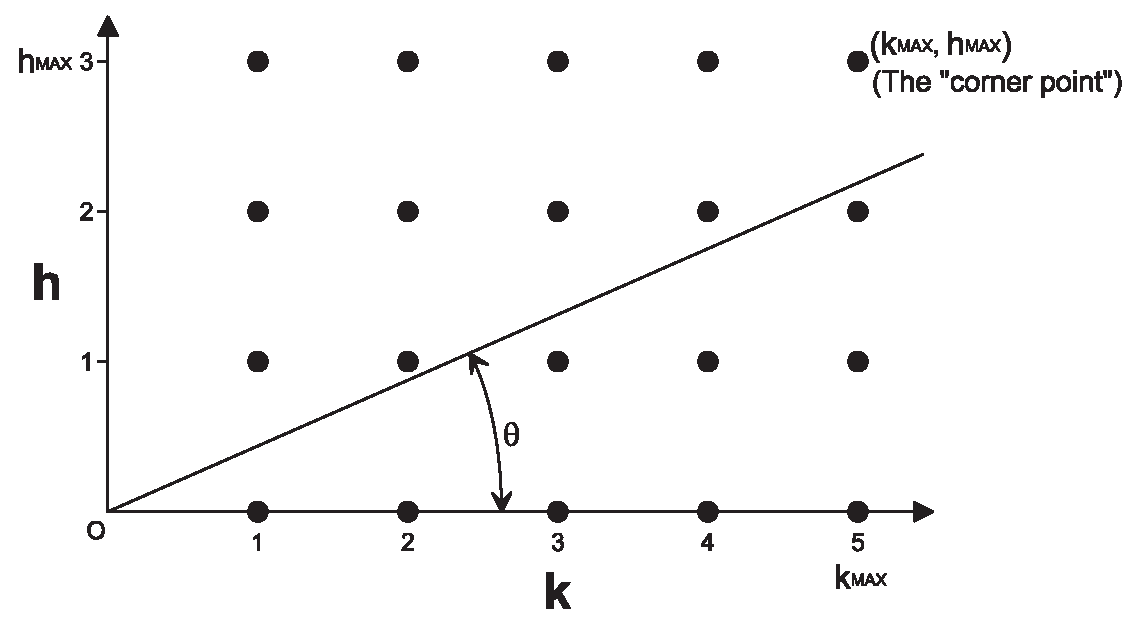
\includegraphics[width=4.6in]{c_rla1/farey01a.eps}
\caption{Graphical Interpretation Of Rational Numbers
         $h/k$ That Can Be Formed With $h \leq h_{MAX}=3$, $k \leq k_{MAX}=5$}
\label{fig:crla1:sfry0:00}
\end{figure}

From the graphical interpretation suggested by Fig.
\ref{fig:crla1:sfry0:00}, the following properties are apparent:

\begin{itemize}
\item The angle of a ray drawn from the origin to the point $(k,h)$
      corresponding to the rational number $h/k$ is $\theta = tan^{-1} \; h/k$.
\item Any integer lattice point on a line from the origin drawn at the
      angle $\theta$ has the value $h/k = tan \; \theta$.  All points
      corresponding to rational numbers with the same value will be on this
      line.
\item A rational number $h/k$ is irreducible if and only if its
      corresponding point $(k,h)$ is directly visible from the origin with
      no intervening points.
\item The Farey series of order $N$, $F_N$, can be formed graphically by
      starting with the set of integer lattice points $(k,h): \; h \in
      \vworkintsetnonneg \wedge 1 \leq k \leq N$, then sweeping a line extended
      from the origin, starting with angle $\theta = 0$, through $0 \leq \theta
      < \pi{}/2$, and recording in order each point directly visible from the
      origin.\footnote{Note that Fig.  \ref{fig:crla1:sfry0:00}, because
      it illustrates the case when $h$ is constrained as well, does not show
      integer lattice points for $h > h_{MAX}$.  If the integer
      lattice shown in Fig.  \ref{fig:crla1:sfry0:00} were extended
      upward, every positive irreducible rational number with
      $k \leq k_{MAX} = 5$ could be found graphically.}
\end{itemize}

Fig.  \ref{fig:crla1:sfry0:01} illustrates the graphical construction
method for $F_5$.  Note that only integer lattice points which are
directly visible from the origin (with no intervening points) are
selected.  (Fig.  \ref{fig:crla1:sfry0:01}, like Fig.
\ref{fig:crla1:sfry0:00}, shows the case of constrained $h$---the integer
lattice should be continued upward to construct $F_5$.)

\begin{figure}
\centering
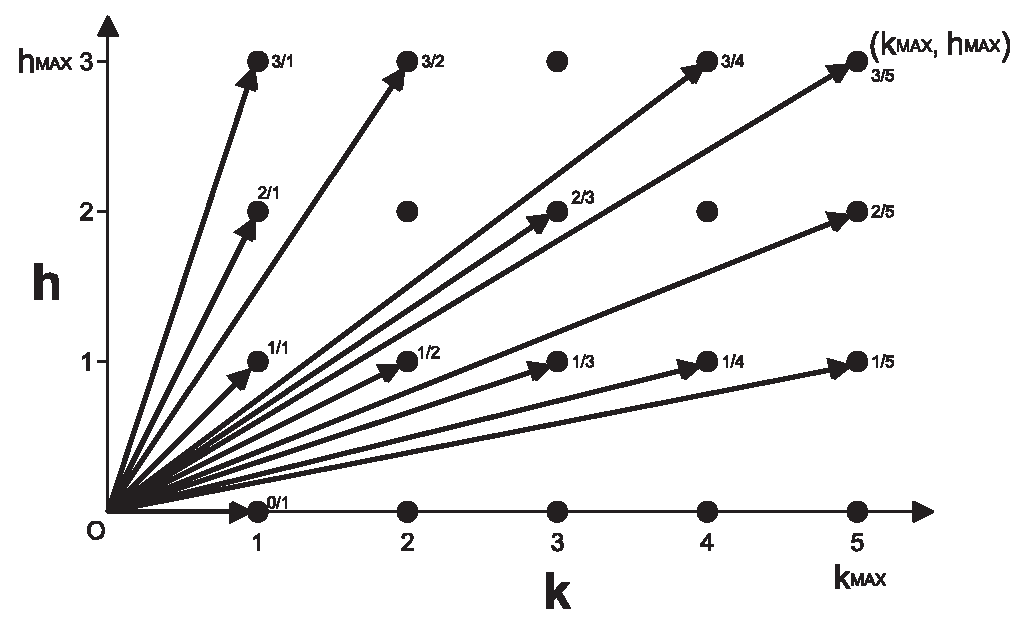
\includegraphics[width=4.6in]{c_rla1/farey01b.eps}
\caption{Graphical Interpretation Of Irreducible Rational Numbers
         $h/k$ That Can Be Formed With $h \leq h_{MAX}=3$, $k \leq k_{MAX}=5$}
\label{fig:crla1:sfry0:01}
\end{figure}

I denote the set of non-negative irreducible rational numbers that can be formed
with $h \leq h_{MAX}$ and $k \leq k_{MAX}$ as $F_{k_{MAX}, h_{MAX}}$\@.
Using this notation, the graphical construction method
depicted in Figure \ref{fig:crla1:sfry0:01} identifies $F_{5,3}$:

\begin{equation}
\label{eq:crla1:sfry0:eq0002a}
F_{5,3}  = \left\{ {\frac{0}{1},\frac{1}{5},\frac{1}{4},
                    \frac{1}{3},\frac{2}{5},\frac{1}{2},
                    \frac{3}{5},\frac{2}{3},\frac{3}{4},
                    \frac{1}{1},\frac{3}{2},\frac{2}{1},
                    \frac{3}{1}} \right\} .
\end{equation}


The ``corner point'' in Figures \ref{fig:crla1:sfry0:00}
and \ref{fig:crla1:sfry0:01}, $k_{MAX}/h_{MAX} = 5/3$, plays a special role:

\begin{itemize}
\item From 0/1 up through the corner point $h_{MAX}/k_{MAX}$,
      the terms are the terms of the Farey series of order
      $k_{MAX}$.
\item From $h_{MAX}/k_{MAX}$ up through $h_{MAX}/1$, the terms
      are the reverse-ordered reciprocals of the terms of the
      Farey series of order $h_{MAX}$\@. (This can be seen
      by transposing the $h$ and $k$ axes of the figures.)
\end{itemize}

The observation about the terms of $F_{5,3}$ that are greater than 3/5 is
important, because it means that if there is a method for finding the
nearest Farey series neighbors to a real number $r_I$ (the case of
only $k$ constrained, $k \leq k_{MAX}$), then there is also a method for finding
the nearest neighbors in $F_{k_{MAX}, h_{MAX}}$ (both $h$ and $k$ constrained).
The method is:

\begin{itemize}
\item If $r_I < k_{MAX}/h_{MAX}$, find the nearest neighbors to $r_I$ in
      $F_{k_{MAX}}$.
\item If $r_I > k_{MAX}/h_{MAX}$, find the nearest neighbors to $1/r_I$
      in $F_{h_{MAX}}$; the reciprocals of those neighbors are the closest
      rational numbers in $F_{k_{MAX}, h_{MAX}}$ to $r_I$.
\end{itemize}

%%%%%%%%%%%%%%%%%%%%%%%%%%%%%%%%%%%%%%%%%%%%%%%%%%%%%%%%%%%%%%%%%%%%%%%%%%%%%%%
%%%%%%%%%%%%%%%%%%%%%%%%%%%%%%%%%%%%%%%%%%%%%%%%%%%%%%%%%%%%%%%%%%%%%%%%%%%%%%%
%%%%%%%%%%%%%%%%%%%%%%%%%%%%%%%%%%%%%%%%%%%%%%%%%%%%%%%%%%%%%%%%%%%%%%%%%%%%%%%
\section{The Continued Fraction Algorithm}
\label{crla1:scfr0}

A \emph{finite simple continued fraction} is a fraction of the form

\begin{equation}
\label{eq:crla1:scfr0:00}
a_0 + \cfrac{1}{a_1 + \cfrac{1}{a_2
    + \cfrac{1}{\;\;\;\;\;\;\;\;\;\;\;\;\;\;\ldots + \cfrac{1}{a_n}}}}
    =
    [a_0; a_1, a_2, \ldots , a_n] ,
\end{equation}

\noindent{}where $a_0 \in \vworkintsetnonneg$ and $a_i \in
\vworkintsetpos$, $i > 0$.  Each integer $a_i$ is called an
\index{continued fraction!element}\emph{element} or \index{continued
fraction!partial quotient}\emph{partial quotient} of the continued
fraction.  To ensure a unique representation, it is required, except in
the case of the continued fraction representation of an integer, that the
final element $a_n$ not be equal to 1.

Continued fractions are unwieldly to write and typeset, so a continued
fraction in the form of (\ref{eq:crla1:scfr0:00}) is written as
$[a_0; a_1, a_2, \ldots , a_n]$.  The separator between $a_0$ and $a_1$ is
a semicolon (`;'), and all other separators are commas (`,').

Continued fractions can be either finite or infinite:

\begin{itemize}
\item A finite continued fraction consists of a finite number of elements
      $[a_0;$ $a_1,$ $a_2,$ $\ldots ,$ $a_n]$\@.  It can be proved that every rational
      number corresponds to a unique finite continued fraction, and that
      every finite continued fraction corresponds to a unique rational number.
\item An infinite continued fraction consists of an infinite number of
      elements $[a_0; a_1, a_2, \ldots]$.  Because every rational number
      corresponds to a finite continued fraction, all irrational numbers have
      infinite continued fraction representations.
\end{itemize}

In engineering work (and due to the general prevalence of computers
and calculators), any $r_I$ to be approximated has a known approximate
numerical value.  Even quantities that are known to be irrational (such
as $\pi$ or $\sqrt{2}$) have a numerical value known to a large number
of significant digits.  For this reason, only the numerical procedure for
obtaining the continued fraction representation of a rational number is
presented (the symbolic procedure is not discussed).  Numerical values
are always rational (for example, 3.1415 is 31,415/10,000).

\index{continued fraction!convergent}The \emph{kth order convergent} of a
continued fraction $[a_0; a_1, \ldots{}, a_n]$ is the irreducible rational
number corresponding to $[a_0; a_1, \ldots{}, a_k]$, $k \leq n$.

An $n$th order continued fraction $[a_0; a_1, \ldots{}, a_n]$ has $n+1$
convergents, $[a_0]$, $[a_0; a_1]$, \ldots{}, and $[a_0; a_1, \ldots{},
a_n]$.  The $k$th order convergent is denoted $s_k$, with numerator $p_k$
and denominator $q_k$.

Algorithm \ref{alg:crla1:scfr0:akgenalg} (below, proof omitted for
brevity) can be used to determine the continued fraction representation
(i.e.  the partial quotients) as well as the convergents of a non-negative
rational number $a/b$\@.

\begin{vworkalgorithmstatementpar}{Continued Fraction Representation and
                                   Convergents of
                                   A Rational Number \mbox{\boldmath $a/b$}}
\label{alg:crla1:scfr0:akgenalg}

\textbf{\emph{Note:}} It is not required that $a/b$ be irreducible.

\begin{alglvl0}
\item $k:=-1$.
\item $divisor_{-1} := a$.
\item $remainder_{-1} := b$.

\item Repeat

\begin{alglvl1}
\item $k := k + 1$.
\item $dividend_k := divisor_{k-1}$.
\item $divisor_k  := remainder_{k-1}$.
\item $a_k :=  dividend_k \; div \; divisor_k$.
\item $remainder_k := dividend_k \; mod \; divisor_k$.
\item If $k=0$, $p_0 = a_0$; else if $k=1$, $p_1 = a_0 a_1 + 1$;
      else $p_i = a_i p_{i-1} + p_{i-2}$.
\item If $k=0$, $q_0 = 1$; else if $k=1$, $q_1 = a_1$;
      else $q_i = a_i q_{i-1} + q_{i-2}$.
\end{alglvl1}

\item Until ($remainder_k = 0$).
\end{alglvl0}
\textbf{\emph{Note:}} The final $s_k = p_k / q_k$ is the irreducible
form of $a/b$.
\end{vworkalgorithmstatementpar}
\vworkalgorithmfooter{}

Convergents have two useful and interesting properties:

\begin{itemize}
\item For each convergent $s_k = p_k/q_k$, there is no rational number
      with a smaller denominator closer to $a/b$\@.\footnote{Table
      \ref{tbl:crla1:sxmp0:01}, part of an example at the end
      of this chapter, provides convergents of $\pi$\@.  It should be
      noted how good the approximations are, even with small denominators,
      due to the average density of rational numbers on the number line\@.
      $s_3$=355/113, for example, has an error on the order of $10^{-7}$\@.
      If this approximation were used to calculate the circumference of the
      earth, the resulting error would be about 11 feet, 2 inches.}
\item Even-ordered convergents are less than $a/b$, and odd-ordered
      convergents are greater than $a/b$; except for the final convergent,
      which is precisely equal to $a/b$.
\end{itemize}

Finally, I present without proof a theorem that indicates how to bracket
a rational number $a/b$ that is not in $F_{k_{MAX}}$ with its two neighbors
in $F_{k_{MAX}}$.

\begin{vworktheoremstatementpar}{Enclosing Neighbors Of \mbox{\boldmath $x \notin F_N$}
                                 In \mbox{\boldmath $F_N$}}
\label{thm:crla1:scfr0:cfenclosingneighbors}
For a non-negative rational
number $a/b$ not in
$F_N$ which has a
continued fraction representation
$[a_0;a_1,a_2,\ldots{} ,a_n]$, the
highest-order convergent $s_k = p_k/q_k$ with $q_k \leq N$ is one
neighbor
to $a/b$ in $F_N$, and the other neighbor in
$F_N$ is

\begin{equation}
\label{eq:crla1:scfr0:thm:cfenclosingneighbors:01}
\frac{{\displaystyle{\left\lfloor {\frac{{N - q_{k - 1} }}{{q_k }}} \right\rfloor}
 p_k  + p_{k - 1} }}{{\displaystyle{\left\lfloor {\frac{{N - q_{k - 1} }}{{q_k }}}
 \right\rfloor} q_k  + q_{k - 1} }}.
\end{equation}
\end{vworktheoremstatementpar}
\begin{vworktheoremproof}
Omitted, as it relies on material not presented for brevity.
\end{vworktheoremproof}
\vworktheoremfooter{}

Theorem \ref{thm:crla1:scfr0:cfenclosingneighbors} can also be applied to
find the Farey neighbors of an $a/b \in F_{k_{MAX}}$.  If
Algorithm \ref{alg:crla1:scfr0:akgenalg} is applied to $a/b$,
(\ref{eq:crla1:scfr0:thm:cfenclosingneighbors:01}) will provide one Farey
neighbor, and (\ref{eq:crla1:sfry0:thm:01:eq01}) through
(\ref{eq:crla1:sfry0:thm:01:eq04}) can be used to provide the other Farey
neighbor\@.  (For brevity, the mathematical basis is not presented.)

Many constants $r_I$ to be approximated are engineering constants based on
measurements or arbitrary conventions, and so are known or accepted to
only a finite number of significant digits.  Such constants are always
rational, and Algorithm \ref{alg:crla1:scfr0:akgenalg} and Theorem
\ref{thm:crla1:scfr0:cfenclosingneighbors} can be applied with no special
consideration.

Some constants, however, are irrational and so have an infinite continued
fraction representation.  The question arises of how to be sure that one
is using enough decimal digits in applying Algorithm
\ref{alg:crla1:scfr0:akgenalg} and Theorem
\ref{thm:crla1:scfr0:cfenclosingneighbors}.  The easiest practical
approach is to confine $r_I$ by an inequality and verify that the Farey
neighbors calculated are the same at both boundaries of the inequality\@.
(It isn't actually necessary to calculate the Farey neighbors to perform
this verification: two rational numbers that have the same highest-order
convergent with $q_k \leq N$ have the same Farey neighbors in $F_N$, but
the \emph{nearest} Farey neighbor may be different for the two rational
numbers.)

Once the two Farey neighbors are calculated, it may be desirable to
determine which is closer to $r_I$.  I'm not aware of a method to do this
other than numerical calculation, although such a method may exist using
higher-order partial quotients or convergents than are used to calculate
the Farey neighbors.


%%%%%%%%%%%%%%%%%%%%%%%%%%%%%%%%%%%%%%%%%%%%%%%%%%%%%%%%%%%%%%%%%%%%%%%%%%%%%%%
%%%%%%%%%%%%%%%%%%%%%%%%%%%%%%%%%%%%%%%%%%%%%%%%%%%%%%%%%%%%%%%%%%%%%%%%%%%%%%%
%%%%%%%%%%%%%%%%%%%%%%%%%%%%%%%%%%%%%%%%%%%%%%%%%%%%%%%%%%%%%%%%%%%%%%%%%%%%%%%
\section{Examples}
\label{crla1:sxmp0}

This section provides examples to illustrate the techniques.

\begin{vworkexamplestatement}
\label{exmp:crla1:sxmp0:01}
Find the best rational approximation to $\pi$ with a denominator not exceeding $2^{24}-1$.
\end{vworkexamplestatement}
\begin{vworkexampleparsection}{Solution} From the problem statement,
$h$ is unconstrained and $k_{MAX}=$16,\-777,\-215.

$2^{24}$ is in the tens of millions (8 digits)\@.  As a crude guess for
how many digits of $\pi$ might lead to unique Farey neighbors for both
ends of an inequality, I will guess 16.

There are numerous websites that provide large numbers of digits of $\pi$\@.
Using 16 digits from a website, one can bound the value of $\pi$:

\begin{equation}
3.141592653589793 < \pi < 3.141592653589794.
\end{equation}

Table \ref{tbl:crla1:sxmp0:01} shows the application of Algorithm
\ref{alg:crla1:scfr0:akgenalg} to find the continued fraction partial
quotients and convergents of $3.141592653589793$\@.  It is only necessary
to continue Algorithm \ref{alg:crla1:scfr0:akgenalg} far enough to establish
the highest-ordered convergent with $q_k \leq k_{MAX}$, and from the table this
is $p_{11}/q_{11}$.

\begin{table}
\caption{Continued Fraction Partial Quotients and Convergents of 3.141592653589793 (Example \ref{exmp:crla1:sxmp0:01})}
\label{tbl:crla1:sxmp0:01}
\begin{center}
\begin{tabular}{|c|c|c|c|c|c|c|}
\hline
\small{Index} & \small{$dividend_k$}      & \small{$divisor_k$}        & \small{$a_k$}   & \small{$remainder_k$}   & \small{$p_k$}      & \small{$q_k$}       \\
\small{($k$)} &                           &                            &                 &                         &                    &                     \\
\hline
\hline
\small{-1}    & \small{N/A}               & \small{3,141,592,}         & \small{N/A}     & \small{1,000,000,}      & \small{N/A}        & \small{N/A}         \\
              &                           & \small{653,589,793}        &                 & \small{000,000,000}     &                    &                     \\
\hline
\small{0}     &  \small{3,141,592}        & \small{1,000,000,}         & \small{3}       & \small{141,592,}        & \small{3}          & \small{1}           \\
              & \small{653,589,793}       & \small{000,000,000}        &                 & \small{653,589,793}     &                    &                     \\
\hline
\small{1}     & \small{1,000,000,}        & \small{141,592,}           & \small{7}       & \small{8,851,}          & \small{22}         & \small{7}           \\
              & \small{000,000,000}       & \small{653,589,793}        &                 & \small{424,871,449}     &                    &                     \\
\hline
\small{2}     & \small{141,592,}          & \small{8,851,}             & \small{15}      & \small{8,821,}          & \small{333}        & \small{106}         \\
              & \small{653,589,793}       & \small{424,871,449}        &                 & \small{280,518,058}     &                    &                     \\
\hline
\small{3}     & \small{8,851,}            & \small{8,821,}             & \small{1}       & \small{30,}             & \small{355}        & \small{113}         \\
              & \small{424,871,449}       & \small{280,518,058}        &                 & \small{144,353,391}     &                    &                     \\
\hline
\small{4}     & \small{8,821,}            & \small{30,}                & \small{292}     & \small{19,}             & \small{103,993}    & \small{33,102}      \\
              & \small{280,518,058}       & \small{144,353,391}        &                 & \small{129,327,886}     &                    &                     \\
\hline
\small{5}     & \small{30,}               & \small{19,}                & \small{1}       & \small{11,}             & \small{104,348}    & \small{33,215}      \\
              & \small{144,353,391}       & \small{129,327,886}        &                 & \small{015,025,505}     &                    &                     \\
\hline
\small{6}     & \small{19,}               & \small{11,}                & \small{1}       & \small{8,}              & \small{208,341}    & \small{66,317}      \\
              & \small{129,327,886}       & \small{015,025,505}        &                 & \small{114,302,381}     &                    &                     \\
\hline
\small{7}     & \small{11,}               & \small{8,}                 & \small{1}       & \small{2,}              & \small{312,689}    & \small{88,532}      \\
              & \small{015,025,505}       & \small{114,302,381}        &                 & \small{900,723,124}     &                    &                     \\
\hline
\small{8}     & \small{8,}                & \small{2,}                 & \small{2}       & \small{2,}              & \small{833,719}    & \small{265,381}     \\
              & \small{114,302,381}       & \small{900,723,124}        &                 & \small{312,856,133}     &                    &                     \\
\hline
\small{9}     & \small{2,}                & \small{2,}                 & \small{1}       & \small{587,866,991}     & \small{1,146,408}  & \small{364,913}     \\
              & \small{900,723,124}       & \small{312,856,133}        &                 &                         &                    &                     \\
\hline
\small{10}    & \small{2,}                & \small{587,866,991}        & \small{3}       & \small{549,255,160}     & \small{4,272,943}  & \small{1,360,120}   \\
              & \small{312,856,133}       &                            &                 &                         &                    &                     \\
\hline
\small{11}    & \small{587,866,991}       & \small{549,255,160}        & \small{1}       & \small{38,611,831}      & \small{5,419,351}  & \small{1,725,033}   \\
\hline
\small{12}    & \small{549,255,160}       & \small{38,611,831}         & \small{14}      & \small{8,689,526}       & \small{80,143,857} & \small{25,510,582}  \\
\hline
\multicolumn{7}{|c|}{\small{Remaining partial quotients and convergents omitted.}} \\
\hline
\end{tabular}
\end{center}
\end{table}

From Theorem \ref{thm:crla1:scfr0:cfenclosingneighbors}, one Farey
neighbor of 3.141592653589793 is

\begin{equation}
s_{11} = \frac{p_{11}}{q_{11}} = \frac{5,\!419,\!351}{1,\!725,\!033} .
\end{equation}

By (\ref{eq:crla1:scfr0:thm:cfenclosingneighbors:01}), the other Farey neighbor is

\begin{eqnarray}
\nonumber{}& \displaystyle{\frac{{\displaystyle{\left\lfloor {\frac{{N - q_{k - 1} }}{{q_k }}} \right\rfloor}
 p_k  + p_{k - 1} }}{{\displaystyle{\left\lfloor {\frac{{N - q_{k - 1} }}{{q_k }}}
 \right\rfloor} q_k  + q_{k - 1} }}}
& \\
& =
\displaystyle{\frac{{\displaystyle{\left\lfloor {\frac{{16,\!777,\!215 - 1,\!360,\!120 }}{{1,\!725,\!033}}} \right\rfloor}
 5,\!419,\!351  + 4,\!272,\!943 }}{{\displaystyle{\left\lfloor {\frac{{16,\!777,\!215 - 1,\!360,\!120 }}{{1,\!725,\!033}}}
 \right\rfloor} 1,\!725,\!033  + 1,\!360,\!120 }}} & \\
\nonumber{}& =
\displaystyle{\frac{\displaystyle{47,\!627,\!751}}{\displaystyle{15,\!160,\!384}}} &
\end{eqnarray}

It can be verified that 3.141592653589794 has the same convergents through
$s_{11} = p_{11}/q_{11}$, so it has the same Farey neighbors as
3.141592653589793\@.  Because $s_{11}$ is an odd-ordered convergent, it is guaranteed to
be greater than $r_I$, establishing the ordering of the Farey neighbors:

\begin{eqnarray}
\nonumber{} & \displaystyle{\frac{47,\!627,\!751}{15,\!160,\!384}} < 3.141592653589793 & \\
            & < \pi < & \\
\nonumber{} & 3.141592653589794 < \displaystyle{\frac{5,\!419,\!351}{1,\!725,\!033}} .
\end{eqnarray}

It can be verified by calculation that the left Farey neighbor is
closer to $\pi$ than the right neighbor, although both are extremely good
approximations (with an error on the order of $10^{-14}$).
\end{vworkexampleparsection}

\begin{vworkexamplestatement}
\label{exmp:crla1:sxmp0:02}
Find the best rational approximation to 1.609344 with a numerator
not exceeding 50,000 and denominator not exceeding
exceeding 60,000.
\end{vworkexamplestatement}
\begin{vworkexampleparsection}{Solution} From the problem statement,
$h_{MAX}=50,\!000$ and $k_{MAX}=60,\!000$.

The corner point (see Fig. \ref{fig:crla1:sfry0:01}, p. \pageref{fig:crla1:sfry0:01})
is $k_{MAX}/h_{MAX} = 1.2$\@.  Since $1.609344 > 1.2$, it is necessary to search
for the Farey neighbors of $1.609344^{-1}$ in $F_{h_{MAX}}$, and the reciprocals
of those neighbors will be the best rational approximations we seek.

Table \ref{tbl:crla1:sxmp0:02} shows the application of Algorithm
\ref{alg:crla1:scfr0:akgenalg} to find the continued fraction partial
quotients and convergents of 1000000/1609344 (the reciprocal of 1.609344).

\begin{table}
\caption{Continued Fraction Partial Quotients and Convergents of $1.609344^{-1}$ (Example \ref{exmp:crla1:sxmp0:02})}
\label{tbl:crla1:sxmp0:02}
\begin{center}
\begin{tabular}{|c|c|c|c|c|c|c|}
\hline
\small{Index} & \small{$dividend_k$}      & \small{$divisor_k$}        & \small{$a_k$}   & \small{$remainder_k$}   & \small{$p_k$}      & \small{$q_k$}       \\
\small{($k$)} &                           &                            &                 &                         &                    &                     \\
\hline
\hline
\small{-1}    & \small{N/A}               & \small{1,000,000}          & \small{N/A}     & \small{1,609.344}       & \small{N/A}        & \small{N/A}         \\
\hline
\small{0}     &  \small{1,000,000}        & \small{1,609344}           & \small{0}       & \small{1,000,000}       & \small{0}          & \small{1}           \\
\hline
\small{1}     & \small{1,609,344,}        & \small{1,000,000}          & \small{1}       & \small{609,344}         & \small{1}          & \small{1}           \\
\hline
\small{2}     & \small{1,000,000}         & \small{609,344}            & \small{1}       & \small{390,656}         & \small{1}          & \small{2}           \\
\hline
\small{3}     & \small{609,344}           & \small{390,656}            & \small{1}       & \small{218,688}         & \small{2}          & \small{3}           \\
\hline
\small{4}     & \small{390,656}           & \small{218,688}            & \small{1}       & \small{171,968}         & \small{3}          & \small{5}           \\
\hline
\small{5}     & \small{218,688}           & \small{171,968}            & \small{1}       & \small{46,720}          & \small{5}          & \small{8}           \\
\hline
\small{6}     & \small{171,968}           & \small{46,720}             & \small{3}       & \small{31,080}          & \small{18}         & \small{29}          \\
\hline
\small{7}     & \small{46,720}            & \small{31,080}             & \small{1}       & \small{14,912}          & \small{23}         & \small{37}          \\
\hline
\small{8}     & \small{31,808}            & \small{14,912}             & \small{2}       & \small{1,984}           & \small{64}         & \small{103}         \\
\hline
\small{9}     & \small{14,912}            & \small{1,984}              & \small{7}       & \small{1,024}           & \small{471}        & \small{758}         \\
\hline
\small{10}    & \small{46,720}            & \small{1,024}              & \small{1}       & \small{960}             & \small{535}        & \small{861}         \\
\hline
\small{11}    & \small{1,024}             & \small{960}                & \small{1}       & \small{64}              & \small{1,006}      & \small{1,619}       \\
\hline
\small{12}    & \small{960}               & \small{64}                 & \small{15}      & \small{0}               & \small{15,625}     & \small{25,146}      \\
\hline
\end{tabular}
\end{center}
\end{table}

Note in Table \ref{tbl:crla1:sxmp0:02} that the final convergent (the reduced
form of 1,000,000/1,609,344), $s_{12} = 15,\!625/25,\!146$, has
$q_{12} < h_{MAX}$, so the reduced form of 1,000,000/1,609,344
is already in $F_{h_{MAX}}$.

It may be helpful to have more choices of a rational number than $1/s_{12}$.  We can use
(\ref{eq:crla1:scfr0:thm:cfenclosingneighbors:01}) to find an adjacent member
of $F_{h_{MAX}}$.  Although $1/s_{12}$ is exactly $r_I$, the same logic mentioned
earlier involving even-numbered and odd-numbered convergents applies.  Even-numbered
convergents (except the final convergent) are less than $r_I$, so the rational number formed by
(\ref{eq:crla1:scfr0:thm:cfenclosingneighbors:01}) will be greater than $s_{12}$.
Applying (\ref{eq:crla1:scfr0:thm:cfenclosingneighbors:01}) yields:

\begin{eqnarray}
\nonumber{}& \displaystyle{\frac{{\displaystyle{\left\lfloor {\frac{{N - q_{k - 1} }}{{q_k }}} \right\rfloor}
 p_k  + p_{k - 1} }}{{\displaystyle{\left\lfloor {\frac{{N - q_{k - 1} }}{{q_k }}}
 \right\rfloor} q_k  + q_{k - 1} }}}
& \\
& =
\displaystyle{\frac{{\displaystyle{\left\lfloor {\frac{{50,\!000 - 1,\!619 }}{{25,\!146}}} \right\rfloor}
 15,\!625  + 1,\!006 }}{{\displaystyle{\left\lfloor {\frac{{50,\!000 - 1,\!619 }}{{25,\!146}}}
 \right\rfloor} 25,\!146  + 1,\!619 }}} & \\
\nonumber{}& =
\displaystyle{\frac{\displaystyle{16,\!631}}{\displaystyle{26,\!765}}} &
\end{eqnarray}

We now have calculated two consecutive terms in $F_{50,\!000}$, $s_{12}$=15,625/25,146 and 16,631/26,765\@.
We can apply (\ref{eq:crla1:sfry0:thm:01:eq03}) and (\ref{eq:crla1:sfry0:thm:01:eq04}) to obtain
the previous term:

\begin{eqnarray}
\nonumber{}h_j  & = & \left\lfloor {\frac{{k_{j + 2}  + N}}{{k_{j + 1} }}}\right\rfloor h_{j + 1}  - h_{j + 2} \\
                & = & \left\lfloor {\frac{{26,\!765  + 50,\!000}}{{25,\!146 }}}\right\rfloor 15,\!625  - 16,\!631 \\
\nonumber{}     & = & 30,\!244
\end{eqnarray}

\begin{eqnarray}
\nonumber{}k_j  & = & \left\lfloor {\frac{{k_{j + 2}  + N}}{{k_{j + 1} }}}\right\rfloor k_{j + 1}  - k_{j + 2} \\
                & = & \left\lfloor {\frac{{26,\!765  + 50,\!000}}{{25,\!146 }}}\right\rfloor 25,\!146  - 26,\!765 \\
\nonumber{}     & = & 48,\!673
\end{eqnarray}

We have determined three consecutive terms of $F_{50,\!000}$:

\begin{equation}
F_{50,\!000} = \left\{ \ldots, \frac{30,\!244}{48,\!673},
\frac{15,\!625}{25,\!146} = s_{12} = 1.609344^{-1},
\frac{16,\!631}{26,\!765}, \ldots \right\}.
\end{equation}

If we take the reciprocals of the terms and reverse the order, we also have determined
three consecutive terms of $F_{50,\!000,60,\!000}$:

\begin{equation}
\label{eq:crla1:sxmp0:02:01}
F_{50,\!000,60,\!000} = \left\{ \ldots, \frac{26,\!765}{16,\!631},
\frac{25,\!146}{15,\!625} = s_{12}^{-1} = 1.609344,
\frac{48,\!673}{30,\!244}, \ldots \right\}.
\end{equation}

All three of the approximations in (\ref{eq:crla1:sxmp0:02:01}) are quite
good.  For most applications, the exact value $r_I = 1/s_{12} =
25,\!146/15,\!625$ would be used.  However, even in the case where $r_I$
can be represented exactly under the constraints, it is possible to
determine neighboring rational approximations.
\end{vworkexampleparsection}



% Chapter: Coding Theory
\chapter{Coding Theory}
\label{ccth0}

%%%%%%%%%%%%%%%%%%%%%%%%%%%%%%%%%%%%%%%%%%%%%%%%%%%%%%%%%%%%%%%%%%%%%%%%%%%%%%%
%%%%%%%%%%%%%%%%%%%%%%%%%%%%%%%%%%%%%%%%%%%%%%%%%%%%%%%%%%%%%%%%%%%%%%%%%%%%%%%
%%%%%%%%%%%%%%%%%%%%%%%%%%%%%%%%%%%%%%%%%%%%%%%%%%%%%%%%%%%%%%%%%%%%%%%%%%%%%%%
\section{Introduction and Overview}
\label{ccth0:siov0}

TBD.



% Chapter: Non-Numerical Algorithms
\chapter{Non-Numerical Algorithms}
\label{cnna0}

%%%%%%%%%%%%%%%%%%%%%%%%%%%%%%%%%%%%%%%%%%%%%%%%%%%%%%%%%%%%%%%%%%%%%%%%%%%%%%%
%%%%%%%%%%%%%%%%%%%%%%%%%%%%%%%%%%%%%%%%%%%%%%%%%%%%%%%%%%%%%%%%%%%%%%%%%%%%%%%
%%%%%%%%%%%%%%%%%%%%%%%%%%%%%%%%%%%%%%%%%%%%%%%%%%%%%%%%%%%%%%%%%%%%%%%%%%%%%%%
\section{Introduction and Overview}
\label{cnna0:siov0}

TBD.



% Chapter: Integer Arithmetic Algorithms and Implementation
\chapter{Integer Arithmetic Algorithms and Implementation}        
\label{caal0}

%%%%%%%%%%%%%%%%%%%%%%%%%%%%%%%%%%%%%%%%%%%%%%%%%%%%%%%%%%%%%%%%%%%%%%%%%%%%%%%
%%%%%%%%%%%%%%%%%%%%%%%%%%%%%%%%%%%%%%%%%%%%%%%%%%%%%%%%%%%%%%%%%%%%%%%%%%%%%%%
%%%%%%%%%%%%%%%%%%%%%%%%%%%%%%%%%%%%%%%%%%%%%%%%%%%%%%%%%%%%%%%%%%%%%%%%%%%%%%%
\section{Introduction}
\label{caal0:sint0}

TBD.




% Chapter: Integer Mathematical Algorithms and Implementation
\chapter{Integer Mathematical Algorithms and Implementation}        
\label{cmal0}

%%%%%%%%%%%%%%%%%%%%%%%%%%%%%%%%%%%%%%%%%%%%%%%%%%%%%%%%%%%%%%%%%%%%%%%%%%%%%%%
%%%%%%%%%%%%%%%%%%%%%%%%%%%%%%%%%%%%%%%%%%%%%%%%%%%%%%%%%%%%%%%%%%%%%%%%%%%%%%%
%%%%%%%%%%%%%%%%%%%%%%%%%%%%%%%%%%%%%%%%%%%%%%%%%%%%%%%%%%%%%%%%%%%%%%%%%%%%%%%
\section{Introduction}
\label{cmal0:sint0}

TBD.




% Chapter: Fixed-Point Arithmetic Algorithms and Implementation
\chapter{Fixed-Point Arithmetic Algorithms and Implementation}        
\label{caal2}

%%%%%%%%%%%%%%%%%%%%%%%%%%%%%%%%%%%%%%%%%%%%%%%%%%%%%%%%%%%%%%%%%%%%%%%%%%%%%%%
%%%%%%%%%%%%%%%%%%%%%%%%%%%%%%%%%%%%%%%%%%%%%%%%%%%%%%%%%%%%%%%%%%%%%%%%%%%%%%%
%%%%%%%%%%%%%%%%%%%%%%%%%%%%%%%%%%%%%%%%%%%%%%%%%%%%%%%%%%%%%%%%%%%%%%%%%%%%%%%
\section{Introduction}
\label{caal2:sint0}

TBD.




% Chapter: Fixed-Point Mathematical Algorithms and Implementation
\chapter{Fixed-Point Mathematical Algorithms and Implementation}        
\label{cmal2}

%%%%%%%%%%%%%%%%%%%%%%%%%%%%%%%%%%%%%%%%%%%%%%%%%%%%%%%%%%%%%%%%%%%%%%%%%%%%%%%
%%%%%%%%%%%%%%%%%%%%%%%%%%%%%%%%%%%%%%%%%%%%%%%%%%%%%%%%%%%%%%%%%%%%%%%%%%%%%%%
%%%%%%%%%%%%%%%%%%%%%%%%%%%%%%%%%%%%%%%%%%%%%%%%%%%%%%%%%%%%%%%%%%%%%%%%%%%%%%%
\section{Introduction}
\label{cmal2:sint0}

TBD.




% Chapter: Real and Floating-Point Arithmetic Algorithms and Implementation
\chapter{Real and Floating-Point Arithmetic Algorithms and Implementation}        
\label{craa0}

%%%%%%%%%%%%%%%%%%%%%%%%%%%%%%%%%%%%%%%%%%%%%%%%%%%%%%%%%%%%%%%%%%%%%%%%%%%%%%%
%%%%%%%%%%%%%%%%%%%%%%%%%%%%%%%%%%%%%%%%%%%%%%%%%%%%%%%%%%%%%%%%%%%%%%%%%%%%%%%
%%%%%%%%%%%%%%%%%%%%%%%%%%%%%%%%%%%%%%%%%%%%%%%%%%%%%%%%%%%%%%%%%%%%%%%%%%%%%%%
\section{Introduction}
\label{craa0:sint0}

TBD.




% Chapter: Real and Floating-Point Mathematical Algorithms and Implementation
\chapter{Real and Floating-Point Mathematical Algorithms and Implementation}        
\label{crma0}

%%%%%%%%%%%%%%%%%%%%%%%%%%%%%%%%%%%%%%%%%%%%%%%%%%%%%%%%%%%%%%%%%%%%%%%%%%%%%%%
%%%%%%%%%%%%%%%%%%%%%%%%%%%%%%%%%%%%%%%%%%%%%%%%%%%%%%%%%%%%%%%%%%%%%%%%%%%%%%%
%%%%%%%%%%%%%%%%%%%%%%%%%%%%%%%%%%%%%%%%%%%%%%%%%%%%%%%%%%%%%%%%%%%%%%%%%%%%%%%
\section{Introduction}
\label{crma0:sint0}

TBD.




% Chapter: Linear Filters and Control System Elements
\chapter{Linear Filters and Control System Elements}
\label{clfc0}

%%%%%%%%%%%%%%%%%%%%%%%%%%%%%%%%%%%%%%%%%%%%%%%%%%%%%%%%%%%%%%%%%%%%%%%%%%%%%%%
%%%%%%%%%%%%%%%%%%%%%%%%%%%%%%%%%%%%%%%%%%%%%%%%%%%%%%%%%%%%%%%%%%%%%%%%%%%%%%%
%%%%%%%%%%%%%%%%%%%%%%%%%%%%%%%%%%%%%%%%%%%%%%%%%%%%%%%%%%%%%%%%%%%%%%%%%%%%%%%
\section{Introduction and Overview}
\label{clfc0:siov0}

TBD.



% Chapter: Non-Linear Filters and Debouncing
\chapter{Non-Linear Filters and Debouncing}
\label{cnlf0}

%%%%%%%%%%%%%%%%%%%%%%%%%%%%%%%%%%%%%%%%%%%%%%%%%%%%%%%%%%%%%%%%%%%%%%%%%%%%%%%
%%%%%%%%%%%%%%%%%%%%%%%%%%%%%%%%%%%%%%%%%%%%%%%%%%%%%%%%%%%%%%%%%%%%%%%%%%%%%%%
%%%%%%%%%%%%%%%%%%%%%%%%%%%%%%%%%%%%%%%%%%%%%%%%%%%%%%%%%%%%%%%%%%%%%%%%%%%%%%%
\section{Introduction and Overview}
\label{cnlf0:siov0}

TBD.



% Chapter: Random and Pseudo-Random Number Generation
\chapter{Random and Pseudo-Random Number Generation}
\label{crng0}

%%%%%%%%%%%%%%%%%%%%%%%%%%%%%%%%%%%%%%%%%%%%%%%%%%%%%%%%%%%%%%%%%%%%%%%%%%%%%%%
%%%%%%%%%%%%%%%%%%%%%%%%%%%%%%%%%%%%%%%%%%%%%%%%%%%%%%%%%%%%%%%%%%%%%%%%%%%%%%%
%%%%%%%%%%%%%%%%%%%%%%%%%%%%%%%%%%%%%%%%%%%%%%%%%%%%%%%%%%%%%%%%%%%%%%%%%%%%%%%
\section{Introduction and Overview}
\label{crng0:siov0}

TBD.



% Chapter: Non-Cryptographic Hashes
\chapter{Non-Cryptographic Hashes}
\label{cnch0}

%%%%%%%%%%%%%%%%%%%%%%%%%%%%%%%%%%%%%%%%%%%%%%%%%%%%%%%%%%%%%%%%%%%%%%%%%%%%%%%
%%%%%%%%%%%%%%%%%%%%%%%%%%%%%%%%%%%%%%%%%%%%%%%%%%%%%%%%%%%%%%%%%%%%%%%%%%%%%%%
%%%%%%%%%%%%%%%%%%%%%%%%%%%%%%%%%%%%%%%%%%%%%%%%%%%%%%%%%%%%%%%%%%%%%%%%%%%%%%%
\section{Introduction and Overview}
\label{cnch0:siov0}

TBD.



% Chapter: Cryptographic Hashes
\chapter{Cryptographic Hashes}
\label{cchs0}

%%%%%%%%%%%%%%%%%%%%%%%%%%%%%%%%%%%%%%%%%%%%%%%%%%%%%%%%%%%%%%%%%%%%%%%%%%%%%%%
%%%%%%%%%%%%%%%%%%%%%%%%%%%%%%%%%%%%%%%%%%%%%%%%%%%%%%%%%%%%%%%%%%%%%%%%%%%%%%%
%%%%%%%%%%%%%%%%%%%%%%%%%%%%%%%%%%%%%%%%%%%%%%%%%%%%%%%%%%%%%%%%%%%%%%%%%%%%%%%
\section{Introduction and Overview}
\label{cchs0:siov0}

TBD.



% Chapter: Symmetric-Key Ciphers and Algorithms
\chapter{Symmetric-Key Ciphers and Algorithms}
\label{cskc0}

%%%%%%%%%%%%%%%%%%%%%%%%%%%%%%%%%%%%%%%%%%%%%%%%%%%%%%%%%%%%%%%%%%%%%%%%%%%%%%%
%%%%%%%%%%%%%%%%%%%%%%%%%%%%%%%%%%%%%%%%%%%%%%%%%%%%%%%%%%%%%%%%%%%%%%%%%%%%%%%
%%%%%%%%%%%%%%%%%%%%%%%%%%%%%%%%%%%%%%%%%%%%%%%%%%%%%%%%%%%%%%%%%%%%%%%%%%%%%%%
\section{Introduction and Overview}
\label{cskc0:siov0}

TBD.



% Chapter: Asymmetric-Key Ciphers and Algorithms
\chapter{Asymmetric-Key Ciphers and Algorithms}
\label{cakc0}

%%%%%%%%%%%%%%%%%%%%%%%%%%%%%%%%%%%%%%%%%%%%%%%%%%%%%%%%%%%%%%%%%%%%%%%%%%%%%%%
%%%%%%%%%%%%%%%%%%%%%%%%%%%%%%%%%%%%%%%%%%%%%%%%%%%%%%%%%%%%%%%%%%%%%%%%%%%%%%%
%%%%%%%%%%%%%%%%%%%%%%%%%%%%%%%%%%%%%%%%%%%%%%%%%%%%%%%%%%%%%%%%%%%%%%%%%%%%%%%
\section{Introduction and Overview}
\label{cakc0:siov0}

TBD.



% Chapter: Miscellaneous Mathematical and Algorithmic Topics
\chapter{Miscellaneous Mathematical and Algorithmic Topics}
\label{cmat0}

%%%%%%%%%%%%%%%%%%%%%%%%%%%%%%%%%%%%%%%%%%%%%%%%%%%%%%%%%%%%%%%%%%%%%%%%%%%%%%%
%%%%%%%%%%%%%%%%%%%%%%%%%%%%%%%%%%%%%%%%%%%%%%%%%%%%%%%%%%%%%%%%%%%%%%%%%%%%%%%
%%%%%%%%%%%%%%%%%%%%%%%%%%%%%%%%%%%%%%%%%%%%%%%%%%%%%%%%%%%%%%%%%%%%%%%%%%%%%%%
\section{Introduction and Overview}
\label{cmat0:siov0}

TBD.



% Part: Library Documentation
\part{Library Documentation}

% Chapter: How to Use UCULIB
\chapter{How to Use \emph{\productbasenameshort{}}}
\label{cuuc0}


%%%%%%%%%%%%%%%%%%%%%%%%%%%%%%%%%%%%%%%%%%%%%%%%%%%%%%%%%%%%%%%%%%%%%%%%%%%%%%%
%%%%%%%%%%%%%%%%%%%%%%%%%%%%%%%%%%%%%%%%%%%%%%%%%%%%%%%%%%%%%%%%%%%%%%%%%%%%%%%
%%%%%%%%%%%%%%%%%%%%%%%%%%%%%%%%%%%%%%%%%%%%%%%%%%%%%%%%%%%%%%%%%%%%%%%%%%%%%%%
\section{Introduction and Overview}
\label{cuuc0:siov0}

TBD.




% Chapter: Utility and Miscellaneous Functions
\chapter{Utility and Miscellaneous Functions}
\label{cnef0}

%%%%%%%%%%%%%%%%%%%%%%%%%%%%%%%%%%%%%%%%%%%%%%%%%%%%%%%%%%%%%%%%%%%%%%%%%%%%%%%
%%%%%%%%%%%%%%%%%%%%%%%%%%%%%%%%%%%%%%%%%%%%%%%%%%%%%%%%%%%%%%%%%%%%%%%%%%%%%%%
%%%%%%%%%%%%%%%%%%%%%%%%%%%%%%%%%%%%%%%%%%%%%%%%%%%%%%%%%%%%%%%%%%%%%%%%%%%%%%%
\section{Introduction and Overview}
\label{cnef0:siov0}

TBD.



% Chapter: Block Memory Functions
\chapter{Block Memory Functions}
\label{cbmf0}

%%%%%%%%%%%%%%%%%%%%%%%%%%%%%%%%%%%%%%%%%%%%%%%%%%%%%%%%%%%%%%%%%%%%%%%%%%%%%%%
%%%%%%%%%%%%%%%%%%%%%%%%%%%%%%%%%%%%%%%%%%%%%%%%%%%%%%%%%%%%%%%%%%%%%%%%%%%%%%%
%%%%%%%%%%%%%%%%%%%%%%%%%%%%%%%%%%%%%%%%%%%%%%%%%%%%%%%%%%%%%%%%%%%%%%%%%%%%%%%
\section{Introduction and Overview}
\label{cbmf0:siov0}

TBD.



% Chapter: Search Functions
\chapter{Search Functions}
\label{csea0}

%%%%%%%%%%%%%%%%%%%%%%%%%%%%%%%%%%%%%%%%%%%%%%%%%%%%%%%%%%%%%%%%%%%%%%%%%%%%%%%
%%%%%%%%%%%%%%%%%%%%%%%%%%%%%%%%%%%%%%%%%%%%%%%%%%%%%%%%%%%%%%%%%%%%%%%%%%%%%%%
%%%%%%%%%%%%%%%%%%%%%%%%%%%%%%%%%%%%%%%%%%%%%%%%%%%%%%%%%%%%%%%%%%%%%%%%%%%%%%%
\section{Introduction and Overview}
\label{csea0:siov0}

TBD.



% Chapter: Sort Functions
\chapter[Sort Functions]
        {Sort Functions}
\chaptermark{Sort Functions}        

\label{csol0}

%%%%%%%%%%%%%%%%%%%%%%%%%%%%%%%%%%%%%%%%%%%%%%%%%%%%%%%%%%%%%%%%%%%%%%%%%%%%%%%
%%%%%%%%%%%%%%%%%%%%%%%%%%%%%%%%%%%%%%%%%%%%%%%%%%%%%%%%%%%%%%%%%%%%%%%%%%%%%%%
%%%%%%%%%%%%%%%%%%%%%%%%%%%%%%%%%%%%%%%%%%%%%%%%%%%%%%%%%%%%%%%%%%%%%%%%%%%%%%%
\section{Introduction and Overview}
\label{csol0:siov0}

TBD.



% Chapter: Array Manipulation Functions
\chapter{Array Manipulation Functions}
\label{cami0}


%%%%%%%%%%%%%%%%%%%%%%%%%%%%%%%%%%%%%%%%%%%%%%%%%%%%%%%%%%%%%%%%%%%%%%%%%%%%%%%
%%%%%%%%%%%%%%%%%%%%%%%%%%%%%%%%%%%%%%%%%%%%%%%%%%%%%%%%%%%%%%%%%%%%%%%%%%%%%%%
%%%%%%%%%%%%%%%%%%%%%%%%%%%%%%%%%%%%%%%%%%%%%%%%%%%%%%%%%%%%%%%%%%%%%%%%%%%%%%%
\section{Introduction and Overview}
\label{cami0:siov0}

TBD.



%% Chapter: Bit-Mapped Set Functions
\chapter{Bit-Mapped Set Functions}        
\label{cbsf0}

%%%%%%%%%%%%%%%%%%%%%%%%%%%%%%%%%%%%%%%%%%%%%%%%%%%%%%%%%%%%%%%%%%%%%%%%%%%%%%%
%%%%%%%%%%%%%%%%%%%%%%%%%%%%%%%%%%%%%%%%%%%%%%%%%%%%%%%%%%%%%%%%%%%%%%%%%%%%%%%
%%%%%%%%%%%%%%%%%%%%%%%%%%%%%%%%%%%%%%%%%%%%%%%%%%%%%%%%%%%%%%%%%%%%%%%%%%%%%%%
\section{Introduction and Overview}
\label{cbsf0:siov0}

TBD.





% Chapter: Vertical Counter Functions
\chapter{Vertical Counter Functions}
\label{cvco0}

%%%%%%%%%%%%%%%%%%%%%%%%%%%%%%%%%%%%%%%%%%%%%%%%%%%%%%%%%%%%%%%%%%%%%%%%%%%%%%%
%%%%%%%%%%%%%%%%%%%%%%%%%%%%%%%%%%%%%%%%%%%%%%%%%%%%%%%%%%%%%%%%%%%%%%%%%%%%%%%
%%%%%%%%%%%%%%%%%%%%%%%%%%%%%%%%%%%%%%%%%%%%%%%%%%%%%%%%%%%%%%%%%%%%%%%%%%%%%%%
\section{Introduction and Overview}
\label{cvco0:siov0}

TBD.



% Chapter: Native Data Type Integer Utility and Arithmetic Functions
\chapter{Native Data Type Integer Utility and Arithmetic Functions}
\label{cafn0}

%%%%%%%%%%%%%%%%%%%%%%%%%%%%%%%%%%%%%%%%%%%%%%%%%%%%%%%%%%%%%%%%%%%%%%%%%%%%%%%
%%%%%%%%%%%%%%%%%%%%%%%%%%%%%%%%%%%%%%%%%%%%%%%%%%%%%%%%%%%%%%%%%%%%%%%%%%%%%%%
%%%%%%%%%%%%%%%%%%%%%%%%%%%%%%%%%%%%%%%%%%%%%%%%%%%%%%%%%%%%%%%%%%%%%%%%%%%%%%%
\section{Introduction and Overview}
\label{cafn0:siov0}



% Chapter: Native Data Type Integer Mathematical Functions
\chapter{Native Data Type Integer Mathematical Functions}
\label{cbaf0}

%%%%%%%%%%%%%%%%%%%%%%%%%%%%%%%%%%%%%%%%%%%%%%%%%%%%%%%%%%%%%%%%%%%%%%%%%%%%%%%
%%%%%%%%%%%%%%%%%%%%%%%%%%%%%%%%%%%%%%%%%%%%%%%%%%%%%%%%%%%%%%%%%%%%%%%%%%%%%%%
%%%%%%%%%%%%%%%%%%%%%%%%%%%%%%%%%%%%%%%%%%%%%%%%%%%%%%%%%%%%%%%%%%%%%%%%%%%%%%%
\section{Introduction and Overview}
\label{cbaf0:siov0}

TBD.




% Chapter: Native Data Type Fixed-Point Utility and Arithmetic Functions
\chapter{Native Data Type Fixed-Point Utility and Arithmetic Functions}
\label{cfpa0}

%%%%%%%%%%%%%%%%%%%%%%%%%%%%%%%%%%%%%%%%%%%%%%%%%%%%%%%%%%%%%%%%%%%%%%%%%%%%%%%
%%%%%%%%%%%%%%%%%%%%%%%%%%%%%%%%%%%%%%%%%%%%%%%%%%%%%%%%%%%%%%%%%%%%%%%%%%%%%%%
%%%%%%%%%%%%%%%%%%%%%%%%%%%%%%%%%%%%%%%%%%%%%%%%%%%%%%%%%%%%%%%%%%%%%%%%%%%%%%%
\section{Introduction and Overview}
\label{cfpa0:siov0}

TBD.




% Chapter: Native Data Type Fixed-Point Mathematical Functions
\chapter{Native Data Type Fixed-Point Mathematical Functions}
\label{cfpa1}

%%%%%%%%%%%%%%%%%%%%%%%%%%%%%%%%%%%%%%%%%%%%%%%%%%%%%%%%%%%%%%%%%%%%%%%%%%%%%%%
%%%%%%%%%%%%%%%%%%%%%%%%%%%%%%%%%%%%%%%%%%%%%%%%%%%%%%%%%%%%%%%%%%%%%%%%%%%%%%%
%%%%%%%%%%%%%%%%%%%%%%%%%%%%%%%%%%%%%%%%%%%%%%%%%%%%%%%%%%%%%%%%%%%%%%%%%%%%%%%
\section{Introduction and Overview}
\label{cfpa1:siov0}

TBD.



% Chapter: Native Data Type Floating-Point Utility and Arithmetic Functions
\chapter{Native Data Type Floating-Point Utility and Arithmetic Functions}
\label{caal1}

%%%%%%%%%%%%%%%%%%%%%%%%%%%%%%%%%%%%%%%%%%%%%%%%%%%%%%%%%%%%%%%%%%%%%%%%%%%%%%%
%%%%%%%%%%%%%%%%%%%%%%%%%%%%%%%%%%%%%%%%%%%%%%%%%%%%%%%%%%%%%%%%%%%%%%%%%%%%%%%
%%%%%%%%%%%%%%%%%%%%%%%%%%%%%%%%%%%%%%%%%%%%%%%%%%%%%%%%%%%%%%%%%%%%%%%%%%%%%%%
\section{Introduction and Overview}
\label{caal1:siov0}

TBD.



% Chapter: Native Data Type Floating-Point Mathematical Functions
\chapter{Native Data Type Floating-Point Mathematical Functions}
\label{cafn1}

%%%%%%%%%%%%%%%%%%%%%%%%%%%%%%%%%%%%%%%%%%%%%%%%%%%%%%%%%%%%%%%%%%%%%%%%%%%%%%%
%%%%%%%%%%%%%%%%%%%%%%%%%%%%%%%%%%%%%%%%%%%%%%%%%%%%%%%%%%%%%%%%%%%%%%%%%%%%%%%
%%%%%%%%%%%%%%%%%%%%%%%%%%%%%%%%%%%%%%%%%%%%%%%%%%%%%%%%%%%%%%%%%%%%%%%%%%%%%%%
\section{Introduction and Overview}
\label{cafn1:siov0}

TBD.



% Chapter: Large Integer Utility and Arithmetic Functions
\chapter[Large Integer Utility and Arithmetic Functions]
        {Large Integer Utility and Arithmetic Functions}

\chaptermark{Large Integer Utility and Arithmetic Functions}

\label{claf0}

%%%%%%%%%%%%%%%%%%%%%%%%%%%%%%%%%%%%%%%%%%%%%%%%%%%%%%%%%%%%%%%%%%%%%%%%%%%%%%%
%%%%%%%%%%%%%%%%%%%%%%%%%%%%%%%%%%%%%%%%%%%%%%%%%%%%%%%%%%%%%%%%%%%%%%%%%%%%%%%
%%%%%%%%%%%%%%%%%%%%%%%%%%%%%%%%%%%%%%%%%%%%%%%%%%%%%%%%%%%%%%%%%%%%%%%%%%%%%%%
\section{Introduction and Overview}
\label{claf0:siov0}

TBD.



% Chapter: Large Integer Mathematical Functions
\chapter[Large Integer Mathematical Functions]
        {Large Integer Mathematical Functions}

\chaptermark{Large Integer Mathematical Functions}

\label{claf1}

%%%%%%%%%%%%%%%%%%%%%%%%%%%%%%%%%%%%%%%%%%%%%%%%%%%%%%%%%%%%%%%%%%%%%%%%%%%%%%%
%%%%%%%%%%%%%%%%%%%%%%%%%%%%%%%%%%%%%%%%%%%%%%%%%%%%%%%%%%%%%%%%%%%%%%%%%%%%%%%
%%%%%%%%%%%%%%%%%%%%%%%%%%%%%%%%%%%%%%%%%%%%%%%%%%%%%%%%%%%%%%%%%%%%%%%%%%%%%%%
\section{Introduction and Overview}
\label{claf1:siov0}

TBD.



% Chapter: Large Fixed-Point Utility and Arithmetic Functions
\chapter{Large Fixed-Point Utility and Arithmetic Functions}
\label{cfpa2}

%%%%%%%%%%%%%%%%%%%%%%%%%%%%%%%%%%%%%%%%%%%%%%%%%%%%%%%%%%%%%%%%%%%%%%%%%%%%%%%
%%%%%%%%%%%%%%%%%%%%%%%%%%%%%%%%%%%%%%%%%%%%%%%%%%%%%%%%%%%%%%%%%%%%%%%%%%%%%%%
%%%%%%%%%%%%%%%%%%%%%%%%%%%%%%%%%%%%%%%%%%%%%%%%%%%%%%%%%%%%%%%%%%%%%%%%%%%%%%%
\section{Introduction and Overview}
\label{cfpa2:siov0}

TBD.




% Chapter: Large Fixed-Point Mathematical Functions
\chapter{Large Fixed-Point Mathematical Functions}
\label{cfpa3}

%%%%%%%%%%%%%%%%%%%%%%%%%%%%%%%%%%%%%%%%%%%%%%%%%%%%%%%%%%%%%%%%%%%%%%%%%%%%%%%
%%%%%%%%%%%%%%%%%%%%%%%%%%%%%%%%%%%%%%%%%%%%%%%%%%%%%%%%%%%%%%%%%%%%%%%%%%%%%%%
%%%%%%%%%%%%%%%%%%%%%%%%%%%%%%%%%%%%%%%%%%%%%%%%%%%%%%%%%%%%%%%%%%%%%%%%%%%%%%%
\section{Introduction and Overview}
\label{cfpa3:siov0}

TBD.



% Chapter: Large Floating-Point Utility and Arithmetic Functions
\chapter[Large Floating-Point Utility and Arithmetic Functions]
        {Large Floating-Point Utility and Arithmetic Functions}

\chaptermark{Large Floating-Point Utility and Arithmetic Functions}

\label{claf2}

%%%%%%%%%%%%%%%%%%%%%%%%%%%%%%%%%%%%%%%%%%%%%%%%%%%%%%%%%%%%%%%%%%%%%%%%%%%%%%%
%%%%%%%%%%%%%%%%%%%%%%%%%%%%%%%%%%%%%%%%%%%%%%%%%%%%%%%%%%%%%%%%%%%%%%%%%%%%%%%
%%%%%%%%%%%%%%%%%%%%%%%%%%%%%%%%%%%%%%%%%%%%%%%%%%%%%%%%%%%%%%%%%%%%%%%%%%%%%%%
\section{Introduction and Overview}
\label{claf2:siov0}

TBD.



% Chapter: Large Floating-Point Mathematical Functions
\chapter[Large Floating-Point Mathematical Functions]
        {Large Floating-Point Mathematical Functions}

\chaptermark{Large Integer Mathematical Functions}

\label{claf3}

%%%%%%%%%%%%%%%%%%%%%%%%%%%%%%%%%%%%%%%%%%%%%%%%%%%%%%%%%%%%%%%%%%%%%%%%%%%%%%%
%%%%%%%%%%%%%%%%%%%%%%%%%%%%%%%%%%%%%%%%%%%%%%%%%%%%%%%%%%%%%%%%%%%%%%%%%%%%%%%
%%%%%%%%%%%%%%%%%%%%%%%%%%%%%%%%%%%%%%%%%%%%%%%%%%%%%%%%%%%%%%%%%%%%%%%%%%%%%%%
\section{Introduction and Overview}
\label{claf3:siov0}

TBD.



% Chapter: Linear Filter Functions
\chapter{Linear Filter and Control System Element Functions}
\label{clfi0}

%%%%%%%%%%%%%%%%%%%%%%%%%%%%%%%%%%%%%%%%%%%%%%%%%%%%%%%%%%%%%%%%%%%%%%%%%%%%%%%
%%%%%%%%%%%%%%%%%%%%%%%%%%%%%%%%%%%%%%%%%%%%%%%%%%%%%%%%%%%%%%%%%%%%%%%%%%%%%%%
%%%%%%%%%%%%%%%%%%%%%%%%%%%%%%%%%%%%%%%%%%%%%%%%%%%%%%%%%%%%%%%%%%%%%%%%%%%%%%%
\section{Introduction and Overview}
\label{clfi0:siov0}

TBD.




% Chapter: Non-Linear Filter Functions
\chapter{Non-Linear Filter Functions}
\label{cnfi0}


%%%%%%%%%%%%%%%%%%%%%%%%%%%%%%%%%%%%%%%%%%%%%%%%%%%%%%%%%%%%%%%%%%%%%%%%%%%%%%%
%%%%%%%%%%%%%%%%%%%%%%%%%%%%%%%%%%%%%%%%%%%%%%%%%%%%%%%%%%%%%%%%%%%%%%%%%%%%%%%
%%%%%%%%%%%%%%%%%%%%%%%%%%%%%%%%%%%%%%%%%%%%%%%%%%%%%%%%%%%%%%%%%%%%%%%%%%%%%%%
\section{Introduction and Overview}
\label{cnfi0:siov0}

TBD.



% Chapter: Pseudo-Random Number Generation Functions
\chapter{Pseudo-Random Number Generation Functions}
\label{crng1}

%%%%%%%%%%%%%%%%%%%%%%%%%%%%%%%%%%%%%%%%%%%%%%%%%%%%%%%%%%%%%%%%%%%%%%%%%%%%%%%
%%%%%%%%%%%%%%%%%%%%%%%%%%%%%%%%%%%%%%%%%%%%%%%%%%%%%%%%%%%%%%%%%%%%%%%%%%%%%%%
%%%%%%%%%%%%%%%%%%%%%%%%%%%%%%%%%%%%%%%%%%%%%%%%%%%%%%%%%%%%%%%%%%%%%%%%%%%%%%%
\section{Introduction and Overview}
\label{crng1:siov0}

TBD.



% Chapter: Non-Cryptographic Hash Functions
\chapter[Non-Cryptographic Hash Functions]
        {Non-Cryptographic Hash Functions}
\chaptermark{Non-Cryptographic Hash Functions}        
\label{ccrc0}

%%%%%%%%%%%%%%%%%%%%%%%%%%%%%%%%%%%%%%%%%%%%%%%%%%%%%%%%%%%%%%%%%%%%%%%%%%%%%%%
%%%%%%%%%%%%%%%%%%%%%%%%%%%%%%%%%%%%%%%%%%%%%%%%%%%%%%%%%%%%%%%%%%%%%%%%%%%%%%%
%%%%%%%%%%%%%%%%%%%%%%%%%%%%%%%%%%%%%%%%%%%%%%%%%%%%%%%%%%%%%%%%%%%%%%%%%%%%%%%
\section{Introduction and Overview}
\label{ccrc0:siov0}

TBD.



% Chapter: Cryptographic Hash Functions
\chapter{Cryptographic Hash Functions}
\label{ccrh0}

%%%%%%%%%%%%%%%%%%%%%%%%%%%%%%%%%%%%%%%%%%%%%%%%%%%%%%%%%%%%%%%%%%%%%%%%%%%%%%%
%%%%%%%%%%%%%%%%%%%%%%%%%%%%%%%%%%%%%%%%%%%%%%%%%%%%%%%%%%%%%%%%%%%%%%%%%%%%%%%
%%%%%%%%%%%%%%%%%%%%%%%%%%%%%%%%%%%%%%%%%%%%%%%%%%%%%%%%%%%%%%%%%%%%%%%%%%%%%%%
\section{Introduction and Overview}
\label{ccrh0:siov0}

TBD.



% Chapter: Symmetric Cipher Functions
\chapter{Symmetric Cipher Functions}
\label{ccip0}

%%%%%%%%%%%%%%%%%%%%%%%%%%%%%%%%%%%%%%%%%%%%%%%%%%%%%%%%%%%%%%%%%%%%%%%%%%%%%%%
%%%%%%%%%%%%%%%%%%%%%%%%%%%%%%%%%%%%%%%%%%%%%%%%%%%%%%%%%%%%%%%%%%%%%%%%%%%%%%%
%%%%%%%%%%%%%%%%%%%%%%%%%%%%%%%%%%%%%%%%%%%%%%%%%%%%%%%%%%%%%%%%%%%%%%%%%%%%%%%
\section{Introduction and Overview}
\label{ccip0:siov0}

TBD.



% Chapter: Asymmetric Cipher Functions
\chapter{Asymmetric Cipher Functions}
\label{ccip1}

%%%%%%%%%%%%%%%%%%%%%%%%%%%%%%%%%%%%%%%%%%%%%%%%%%%%%%%%%%%%%%%%%%%%%%%%%%%%%%%
%%%%%%%%%%%%%%%%%%%%%%%%%%%%%%%%%%%%%%%%%%%%%%%%%%%%%%%%%%%%%%%%%%%%%%%%%%%%%%%
%%%%%%%%%%%%%%%%%%%%%%%%%%%%%%%%%%%%%%%%%%%%%%%%%%%%%%%%%%%%%%%%%%%%%%%%%%%%%%%
\section{Introduction and Overview}
\label{ccip1:siov0}

TBD.



% Part: Developer and Contributor Information
\part{Developer and Contributor Information}

% Chapter: Library Development and Modification Procedures
\chapter{Library Development and Modification Procedures}
\label{cbpc0}


%%%%%%%%%%%%%%%%%%%%%%%%%%%%%%%%%%%%%%%%%%%%%%%%%%%%%%%%%%%%%%%%%%%%%%%%%%%%%%%
%%%%%%%%%%%%%%%%%%%%%%%%%%%%%%%%%%%%%%%%%%%%%%%%%%%%%%%%%%%%%%%%%%%%%%%%%%%%%%%
%%%%%%%%%%%%%%%%%%%%%%%%%%%%%%%%%%%%%%%%%%%%%%%%%%%%%%%%%%%%%%%%%%%%%%%%%%%%%%%
\section{Generating Library Source Code from Templates}
\label{cbpc0:sgsc0}

TBD.





% Part: Appendices, Bibliography, and Index 
\part{Appendices, Bibliography, and Index}

%Mark the start of appendices.  This causes numbering to be with letters
%instead of numbers.
\appendix

%Glossary of Terms
\chapter{Glossary Of Terms}
\markboth{GLOSSARY OF TERMS}{GLOSSARY OF TERMS}

\label{cglo0}

\begin{vworktermglossaryenum}


\item \index{set!cardinality}\textbf{cardinality}

      The number of elements in a set, denoted $n( \cdot )$. 
      \emph{Example:} $n( \{ 12 , 29 , 327 \} ) = 3$.  

\item \index{coprime}\textbf{coprime}

      Having no prime factors in common.
      \emph{Example:} 6 and 7 are coprime, whereas 6 and 8 are not coprime.  


\end{vworktermglossaryenum}


%
%Glossary of Mathematical Notation
\chapter{Glossary Of Mathematical And Other Notation}
\markboth{GLOSSARY OF MATHEMATICAL NOTATION}{GLOSSARY OF MATHEMATICAL NOTATION}
\label{cglo1}

%%%%%%%%%%%%%%%%%%%%%%%%%%%%%%%%%%%%%%%%%%%%%%%%%%%%%%%%%%%%%%%%%%%%%%%%%%%%%%%
%%%%%%%%%%%%%%%%%%%%%%%%%%%%%%%%%%%%%%%%%%%%%%%%%%%%%%%%%%%%%%%%%%%%%%%%%%%%%%%
%%%%%%%%%%%%%%%%%%%%%%%%%%%%%%%%%%%%%%%%%%%%%%%%%%%%%%%%%%%%%%%%%%%%%%%%%%%%%%%

\section*{General}

\begin{vworkmathtermglossaryenum}

\item \index{divides}%
      \mbox{\boldmath $ \vworkdivides $}

      $a \vworkdivides b$, 
      read ``\emph{$a$ divides $b$}'', denotes that $b/a$ has no remainder.
      Equivalently,
      $(a \vworkdivides b) \Rightarrow (\exists c \in \vworkintset{}, b = ac)$.

\item \index{divides}%
      \mbox{\boldmath $ \vworknotdivides $}

      $a \vworknotdivides b$, 
      read ``\emph{$a$ does not divide $b$}'', denotes that $b/a$ has a reminder.
      Equivalently,
      $(a \vworknotdivides b) \Rightarrow (\nexists c \in \vworkintset{}, b = ac)$.

\item \index{floor function}%
      \mbox{\boldmath $ \lfloor \cdot \rfloor $}

      The \emph{floor} function.  $\lfloor x \rfloor$ is the largest
      integer not larger than $x$.

\item \index{ceiling function}%
      \mbox{\boldmath $\lceil \cdot \rceil$ }

      The \emph{ceiling} function.
      $\lceil x \rceil$
      is the smallest integer not smaller than $x$.
\end{vworkmathtermglossaryenum}

%%%%%%%%%%%%%%%%%%%%%%%%%%%%%%%%%%%%%%%%%%%%%%%%%%%%%%%%%%%%%%%%%%%%%%%%%%%%%%%
%%%%%%%%%%%%%%%%%%%%%%%%%%%%%%%%%%%%%%%%%%%%%%%%%%%%%%%%%%%%%%%%%%%%%%%%%%%%%%%
%%%%%%%%%%%%%%%%%%%%%%%%%%%%%%%%%%%%%%%%%%%%%%%%%%%%%%%%%%%%%%%%%%%%%%%%%%%%%%%
%
%\section*{Usage Of English And Greek Letters}
%
%\begin{vworkmathtermglossaryenum}
%
%\item \mbox {\boldmath $a/b$}
%
%      An arbitrary \index{rational number}rational number.
%
%\item \mbox {\boldmath $ F_N $}
%
%      The \index{Farey series}Farey 
%      series of order $N$.  The Farey series is the
%      ordered set of irreducible rational numbers 
%          in [0,1] with a
%      denominator not larger than $N$.
%
%\item \mbox {\boldmath $F_{k_{MAX}, \overline{h_{MAX}}}$}
%      
%          \index{FKMAXHMAX@$F_{k_{MAX}, \overline{h_{MAX}}}$}
%          The ordered set of irreducible rational numbers
%          $h/k$ subject to the constraints $0 \leq h \leq h_{MAX}$
%          and $1 \leq k \leq h_{MAX}$.  
%%         (See Section \cfryzeroxrefhyphen{}\ref{cfry0:schk0}.)
%
%
%\item \mbox{\boldmath $H/K$}, \mbox{\boldmath $h/k$},
%      \mbox{\boldmath $h'/k'$}, \mbox{\boldmath $h''/k''$},
%      \mbox{\boldmath $h_i/k_i$}
%
%      Terms in a Farey series of order $N$.
%
%\item \mbox{\boldmath $r_A$}
%
%      The rational number $h/k$ used to approximate
%      an arbitrary real number $r_I$.
%
%\item \mbox{\boldmath $r_I$}
%
%      The real number, which may or may not be rational,
%      which is to be approximated by a rational number
%      $r_A = h/k$.
%
%\item \textbf{reduced}
%
%      See \emph{irreducible}.
%
%\item \mbox{\boldmath $s_k = p_k/q_k$}
%
%      The $k$th convergent of a continued fraction.
%
%\item \mbox{\boldmath $x_{MAX}$}
%
%      The largest element of the domain for which the
%      behavior of an approximation must be guaranteed.
%      In this paper, most derivations assume
%      that $x \in [0, x_{MAX}]$, $x_{MAX} \in \vworkintsetpos{}$.
%\end{vworkmathtermglossaryenum}

%%%%%%%%%%%%%%%%%%%%%%%%%%%%%%%%%%%%%%%%%%%%%%%%%%%%%%%%%%%%%%%%%%%%%%%%%%%%%%%
%%%%%%%%%%%%%%%%%%%%%%%%%%%%%%%%%%%%%%%%%%%%%%%%%%%%%%%%%%%%%%%%%%%%%%%%%%%%%%%
%%%%%%%%%%%%%%%%%%%%%%%%%%%%%%%%%%%%%%%%%%%%%%%%%%%%%%%%%%%%%%%%%%%%%%%%%%%%%%%

%\section*{Bitfields And Portions Of Integers}
%
%\begin{vworkmathtermglossaryenum}
%\item \mbox{\boldmath $a_{b}$}
%
%      The $b$th bit of the integer $a$.  Bits are numbered with the
%      least significant bit ``0'', and consecutively through 
%      ``$n-1$'', where $n$ is the total number of bits.
%
%      In general, if $p$ is an $n$-bit unsigned integer,
%
%      \begin{equation}
%      \nonumber p = \sum_{i=0}^{n-1} 2^i p_i .
%      \end{equation}
%
%\item \mbox{\boldmath $a_{c:b}$}
%
%      The integer consisting of the $b$th through the
%      $c$th bits of the integer $a$.  Bits are numbered with the
%      least significant bit ``0'', and consecutively through 
%      ``$n-1$'', where $n$ is the total number of bits.
%
%      For example, if $p$ is a 24-bit unsigned integer, then
%
%      \begin{equation}
%      \nonumber p = 2^{16}p_{23:16} + 2^{8}p_{15:8} + p_{7:0} .
%      \end{equation}
%
%\item \mbox{\boldmath $a_{[b]}$}
%
%      The $b$th word of the integer $a$.  Words are numbered 
%      with the
%      least significant word ``0'', and consecutively through 
%      ``$n-1$'', where $n$ is the total number of words.
%
%      In general, if $p$ is an $n$-word unsigned integer 
%      and $z$ is the wordsize in bits,
%
%      \begin{equation}
%      \nonumber p = \sum_{i=0}^{n-1} 2^{iz} p_i .
%      \end{equation}
%
%\item \mbox{\boldmath $a_{[c:b]}$}
%
%      The integer consisting of the $b$th through the
%      $c$th word of the integer $a$.  Words are numbered with the
%      least significant word ``0'', and consecutively through 
%      ``$n-1$'', where $n$ is the total number of words.
%
%      For example, if $p$ is a 24-word unsigned integer and
%      $z$ is the wordsize in bits, then
%
%      \begin{equation}
%      \nonumber p = 2^{16z}p_{[23:16]} + 2^{8z}p_{[15:8]} + p_{[7:0]} .
%      \end{equation}
%
%\end{vworkmathtermglossaryenum}

%%%%%%%%%%%%%%%%%%%%%%%%%%%%%%%%%%%%%%%%%%%%%%%%%%%%%%%%%%%%%%%%%%%%%%%%%%%%%%%
%%%%%%%%%%%%%%%%%%%%%%%%%%%%%%%%%%%%%%%%%%%%%%%%%%%%%%%%%%%%%%%%%%%%%%%%%%%%%%%
%%%%%%%%%%%%%%%%%%%%%%%%%%%%%%%%%%%%%%%%%%%%%%%%%%%%%%%%%%%%%%%%%%%%%%%%%%%%%%%

%\section*{Matrices And Vectors}
%
%\begin{vworkmathtermglossaryenum}
%
%\item \mbox{\boldmath $0$}
%
%      $\mathbf{0}$ (in bold face) is used to denote either a vector or matrix
%      populated with all zeroes.  Optionally, in cases where the context is not clear
%      or where there is cause to highlight the dimension, $\mathbf{0}$ may be subscripted
%      to indicate the dimension, i.e. 
%      
%      \begin{equation}
%      \nonumber
%      \mathbf{0}_3 = \left[\begin{array}{c} 0 \\ 0 \\ 0 \end{array}\right]
%      \end{equation}
%
%      \begin{equation}
%      \nonumber
%      \mathbf{0}_{3 \times 2} = \left[\begin{array}{cc} 0&0 \\ 0&0 \\ 0&0 \end{array}\right]
%      \end{equation}
%
%\item \mbox{\boldmath $I$}
%
%      $I$ is used to denote the square identity matrix (the matrix with all
%      elements 0 except elements on the diagonal which are 1).
%      Optionally, in cases where the context is not clear
%      or where there is cause to highlight the dimension, $I$ may be subscripted
%      to indicate the dimension, i.e. 
%      
%      \begin{equation}
%      \nonumber
%      I = I_3 = I_{3 \times 3} = \left[\begin{array}{ccc} 1&0&0 \\ 0&1&0 \\ 0&0&1 \end{array}\right]
%      \end{equation}
%
%\end{vworkmathtermglossaryenum}


%%%%%%%%%%%%%%%%%%%%%%%%%%%%%%%%%%%%%%%%%%%%%%%%%%%%%%%%%%%%%%%%%%%%%%%%%%%%%%%
%%%%%%%%%%%%%%%%%%%%%%%%%%%%%%%%%%%%%%%%%%%%%%%%%%%%%%%%%%%%%%%%%%%%%%%%%%%%%%%
%%%%%%%%%%%%%%%%%%%%%%%%%%%%%%%%%%%%%%%%%%%%%%%%%%%%%%%%%%%%%%%%%%%%%%%%%%%%%%%

\section*{Sets}

\begin{vworkmathtermglossaryenum}

\item \index{set!cardinality}\mbox{\boldmath $n( \cdot )$}

      The \emph{cardinality} of a set (the
      number of elements in the set).

\end{vworkmathtermglossaryenum}

%%%%%%%%%%%%%%%%%%%%%%%%%%%%%%%%%%%%%%%%%%%%%%%%%%%%%%%%%%%%%%%%%%%%%%%%%%%%%%%
%%%%%%%%%%%%%%%%%%%%%%%%%%%%%%%%%%%%%%%%%%%%%%%%%%%%%%%%%%%%%%%%%%%%%%%%%%%%%%%
%%%%%%%%%%%%%%%%%%%%%%%%%%%%%%%%%%%%%%%%%%%%%%%%%%%%%%%%%%%%%%%%%%%%%%%%%%%%%%%

%\section*{Sets Of Numbers}
%
%\begin{vworkmathtermglossaryenum}
%
%\item \mbox{\boldmath $\vworkintsetpos$}
%
%      The 
%      \index{natural number}
%      \index{N@$\vworkintsetpos$}
%      set of positive integers (natural numbers).
%
%\item \mbox{\boldmath $\vworkratset$}
%
%      The 
%      \index{rational number}
%      \index{Q@$\vworkratset$}
%      set of rational numbers.
%
%\item \mbox{\boldmath $\vworkratsetnonneg$}
%
%      The 
%      \index{rational number}
%      \index{Q+@$\vworkratsetnonneg$}
%      set of non-negative rational numbers.
%
%\item \mbox{\boldmath $\vworkrealset$}
%
%      The 
%      \index{real number}
%      \index{R@$\vworkrealset$}
%      set of real numbers.
%
%\item \mbox{\boldmath $\vworkrealsetnonneg$}
%
%      The 
%      \index{real number}
%      \index{R+@$\vworkrealsetnonneg$}
%      set of non-negative real numbers.
%
%\item \mbox{\boldmath $\vworkintset$}
%
%      The 
%      \index{integer}
%      \index{Z@$\vworkintset$}
%      set of integers.
%
%\item \mbox{\boldmath $\vworkintsetnonneg$}
%
%      The 
%      \index{integer}
%      \index{Z+@$\vworkintsetnonneg$}
%      set of non-negative integers.
%
%\end{vworkmathtermglossaryenum}


%
%Bibliography
\cleardoublepage
\addcontentsline{toc}{chapter}{Bibliography}
%Legend
%    b - book
%    c - company
%    d - document
%    i - individual, i.e. person
%    n - newsgroup
%    p - paper
%    s - software, software distributions
%    w - web page.
%
%%%%%%%%%%%%%%%%%%%%%%%%%%%%%%%%%%%%%%%%%%%%%%%%%%%%%%%%%%%%%%%%%%%%%%%%%%
\chapter*{Bibliography}

\markboth{BIBLIOGRAPHY}{BIBLIOGRAPHY}

\newcounter{custombibcounter}

\nocite{*}

%%%%%%%%%%%%%%%%%%%%%%%%%%%%%%%%%%%%%%%%%%%%%%%%%%%%%%%%%%%%%%%%%%%%%%%%%%
%
%\section*{Two-Factor Authentication Vendors}
%\index{two-factor authentication}
%
%\begin{thecustombibliography}{9999}
%
%\bibitem{bibref:c:cryptocardcorporation}
%CryptoCard Corporation,\index{CryptoCard Corporation}\\
%\texttt{http://www.cryptocard.com}
%
%\end{thecustombibliography}
%
%
%%%%%%%%%%%%%%%%%%%%%%%%%%%%%%%%%%%%%%%%%%%%%%%%%%%%%%%%%%%%%%%%%%%%%%%%%%
%
%\section*{Corporations and Organizations}
%
%\begin{thecustombibliography}{9999}
%
%\bibitem{bibref:c:cosmicsoftware}
%Cosmic Software\index{Cosmic Software}\\
%\texttt{http://www.cosmic-us.com}
%
%\end{thecustombibliography}
%
%%%%%%%%%%%%%%%%%%%%%%%%%%%%%%%%%%%%%%%%%%%%%%%%%%%%%%%%%%%%%%%%%%%%%%%%%%

%\section*{Individuals}
%
%\begin{thecustombibliography}{9999}
%
%\bibitem{bibref:i:davidtashley}
%David T. Ashley,\index{Ashley, David T.}
%E-mail: \texttt{dashley@gmail.com}
%
%\bibitem{bibref:i:johnbibo}
%John Bibo,\index{Bibo, John}
%E-mail: \texttt{jbibo@cosmic-us.com}
%
%\bibitem{bibref:i:mikeburns}
%Michael Burns,\index{Burns, Michael}
%E-mail: \texttt{mjb@cosmic-us.com}
%
%\end{thecustombibliography}

%%%%%%%%%%%%%%%%%%%%%%%%%%%%%%%%%%%%%%%%%%%%%%%%%%%%%%%%%%%%%%%%%%%%%%%%%%


%\subsection*{Mathematical Philosophy Books}
%
%\begin{thecustombibliography}{9999}
%
%\bibitem{bibref:b:mathematiciansapology:1940}
%G. H. Hardy,
%\newblock{\em A Mathematician's Apology}, ISBN 0-521-42706-1 (Paperback),
%Cambridge University Press.
%
%\end{thecustombibliography}

%%%%%%%%%%%%%%%%%%%%%%%%%%%%%%%%%%%%%%%%%%%%%%%%%%%%%%%%%%%%%%%%%%%%%%%%%%

%\subsection*{Mathematicians (Amateur And Professional)}
%
%\begin{thecustombibliography}{9999}
%
%\bibitem{bibref:i:davideppstein}
%David Eppstein,\index{Eppstein, David}
%E-mail: \texttt{eppstein@ics.uci.edu}
%
%\end{thecustombibliography}

%%%%%%%%%%%%%%%%%%%%%%%%%%%%%%%%%%%%%%%%%%%%%%%%%%%%%%%%%%%%%%%%%%%%%%%%%%

\section*{Books}

\begin{thecustombibliography}{9999}
%
\bibitem{bibref:b:LamportLaTeX}
\index{Lamport, Leslie}\index{LaTeX@\emph{\LaTeX{}}}Leslie Lamport,
\newblock{\em \LaTeX{}: A Document Preparation System},
Addison-Wesley, 1994, 1985; ISBN 0-201-52983-1.

\bibitem{bibref:b:TaocpVolume2}
\index{Knuth, Donald E.}Donald E. Knuth,
\newblock{\em The Art of Computer Programming, Third Edition, Volume 2 / Seminumerical Algorithms},
Addison-Wesley, 1997; ISBN 0-201-89684-2.
%
%\bibitem{bibref:b:KhinchinClassic}
%A. Ya. Khinchin, \index{Khinchin, A. Ya.}
%\newblock{\em Continued Fractions}, University Of
%Chicago Press, 1964; Library Of Congress Catalog Card
%Number 64-15819.
%
%\bibitem{bibref:b:OldsClassic}
%C. D. Olds,
%\newblock{\em Continued Fractions},
%Randam House, 1963,
%Library Of Congress Catalog Card Number 61-12185.
%
\end{thecustombibliography}

%%%%%%%%%%%%%%%%%%%%%%%%%%%%%%%%%%%%%%%%%%%%%%%%%%%%%%%%%%%%%%%%%%%%%%%%%%
\section*{Individuals}


%%%%%%%%%%%%%%%%%%%%%%%%%%%%%%%%%%%%%%%%%%%%%%%%%%%%%%%%%%%%%%%%%%%%%%%%%%

\section*{Websites and Web Pages}

\begin{thecustombibliography}{9999}

\bibitem{bibref:w:gmplibhomepage}
\index{GMP Library@\emph{GMP Library}}GMP Library Home Page,
\texttt{https://gmplib.org/}

\bibitem{bibref:w:miktexhomepage}
\index{MiKTeX@\emph{MiK\TeX{}}}\emph{MiK\TeX{}} Home Page,
\texttt{https://miktex.org/}

\bibitem{bibref:w:wikipedialowpassfilter}
\index{low-pass filter}Low-Pass Filter,
\texttt{http://en.wikipedia.org/wiki/Low-pass\_filter}

\end{thecustombibliography}


%
%Index Must Be Formed At This Directory Level
\cleardoublepage
\addcontentsline{toc}{chapter}{Index}
\printindex
%
\end{document}

%================================================================================
%The information below is from https://www.texfaq.org/FAQ-runheadtoobig.  I'm
%keeping it here because this situation comes up frequently.
%--------------------------------------------------------------------------------
%My section title is too wide for the page header
%--------------------------------------------------------------------------------
%By default, LaTeX sectioning commands make the chapter or section title
%available for use by page headers and the like. Page headers operate in a rather
%constrained area, and it�s common for titles too be too big to fit: the LaTeX
%sectioning commands therefore take an optional argument:
%
%\section[short title]{full title}
%
%If the �short title� is present, it is used both for the table of contents and
%for the page heading. The usual answer to people who complain that their title
%is too big for the running head is to suggest that they the optional argument.
%
%However, using the same text for the table of contents as for the running head
%may also be unsatisfactory: if your chapter titles are seriously long (like those
%of a Victorian novel), a valid and rational scheme is to have a shortened table
%of contents entry, and a really terse entry in the running head.
%
%One of the problems is the tendency of page headings to be set in capitals
%(which take up more space); so why not set headings as written for �ordinary�
%reading? It�s not possible to do so with unmodified LaTeX, but the fancyhdr
%package provides a command \nouppercase for use in its header (and footer)
%lines to suppress LaTeX�s uppercasing tendencies. Classes in the KOMA-script
%bundle don�t uppercase in the first place.
%
%In fact, the sectioning commands use �mark� commands to pass information to the
%page headers. For example, \chapter uses \chaptermark, \section uses
%\sectionmark, and so on. With this knowledge, one can achieve a three-layer
%structure for chapters:
%
%\chapter[middling version]{verbose version}
%\chaptermark{terse version}
%
%which should supply the needs of every taste.
%
%Chapters, however, have it easy: hardly any book design puts a page header on
%a chapter start page. In the case of sections, one has typically to take account
%of the nature of the \*mark commands: the thing that goes in the heading is the
%first mark on the page (or, failing any mark, the last mark on any previous
%page). As a result the recipe for sections is more tiresome:
%
%\section[middling version]{verbose version%
%              \sectionmark{terse version}}
%\sectionmark{terse version}
%
%(the first \sectionmark deals with the header of the page the \section command
%falls on, and the second deal with subsequent pages; note that here, you need the 
%ptional argument to \section, even if �middling version� is in fact the same text
%as �long version�.)
%
%A similar arrangement is necessary even for chapters if the class you�re using is
%odd enough that it puts a page header on a chapter�s opening page.
%
%Note that the titlesec package manages the running heads in a completely different
%fashion; for example, you can use the optional argument of sectioning commands
%for page headers, only, by loading the package as:
%
%\usepackage[toctitles]{titlesec}
%
%The package documentation offers other useful techniques in this area.
%
%The memoir class avoids all the silliness by providing an extra optional
%argument for chapter and sectioning commands, for example:
%
%\section[middling version][terse version]{verbose version}
%
%As a result, it is always possible for users of memoir to tailor the header text to
%fit, with very little trouble.
%================================================================================
%It was discovered that using \index{key@value} entries within footnotes is
%if "value" is formatted.  An additional space was inserted in the .idx file,
%causing the index entry generated from within a footnote to be different than
%the others (and to be listed separately in the index).
%
%Here is the original problematic text:
%    I define \index{limb size}\emph{limb size}\footnote{The terms \emph{limb} 
%    and \emph{limb size} come from \index{GMP Library@\emph{GMP Library}}%
%    \emph{The GMP Library} \cite{bibref:w:gmplibhomepage}.} as the 
%    number of bits in what Knuth calls $w$ (from the quote above).  In 
%
%Here is the line in the .idx file with the extra space:
%    \indexentry{GMP Library@\emph  {GMP Library}}{8}
%
%Here is a web page that describes the problem and a possible workaround.  (My
%workaround, for now is not to use index entries in footnotes.  A second workaround
%might to be to put the \index entry with the footnoted text, rolling the dice that
%the footnote will end up on the same page as the referring number, which it usually
%does.)
%    https://tex.stackexchange.com/questions/145309/index-in-footnode-different-from-index-in-main-text
%
%Here is the most meaningful text from the URL above (in case it disappears):
%    The problem is that \index tries hard not to tokenize its argument too
%    early; but when the \index command appears in the argument to another
%    command (in this case \footnote, the tokenization has already been done.)
%    Thus in the .idx file you get two non matching entries, one with
%
%        @\textit{De Malignitate Erodoti}!
%
%    and the other one with
%
%        @\textit  {De Malignitate Erodoti}!
%
%    A workaround is to always tokenize:
%
%        \newcommand{\indexp}[1]{\index[p]{#1}}
%
%    and using \indexp instead of \index[p].
%================================================================================

